\input{preamble.tex}

\title{1955SCC - Projeto e Análise de Algoritmos}

\institute{Universidade Estadual Paulista Júlio de Mesquita Filho}

\author{Prof. MSc. André Furlan - andre.furlan@unesp.br}

\logo{\includegraphics[height=1cm]{unesp.png}}
\date{\the\year}

\newcommand{\apontar}[2]{
	\underset{\underset{#1}{\uparrow}}{\mathbf{#2}}
}

\begin{document}
	
	\frame{\titlepage}
	
	\section{Apresentação}
		\begin{frame}
	\frametitle{Introdução}
	
	\only<1>{
		\framesubtitle{Bibliografia recomendada}
		\begin{itemize}
			\item KLEINBERG, J., TARDOS, E.; Algorithm Design, Addison-Weslwy, 2005.
			\item CORMEN, T. H., LEISERSON, C. E., RIVEST, R. L., STEIN, C.;
			\item Introduction to	Algorithms, 3rd Edition, The MIT Press, 2009.
			\item SKIENA, S. S., The algorithm design manual, Springer, 2010.
		\end{itemize}
	}

	\only<2>{		
		\framesubtitle{Objetivos e ementa}
		\par Espera-se que ao final do semestre o aluno domine as técnicas para análise de algoritmos, envolvendo o comportamento assintótico de sua execução e de sua eficiência na solução de problemas específicos.
		Espera-se também, que o mesmo tenha condições de julgar e escolher as melhores alternativas, tanto do ponto de vista de tempo como espaço, para algoritmos aplicados em	problemas reais.
	}

	\only<3>{		
		\framesubtitle{Conteúdo}
		\begin{itemize}
			\item Revisão de álgebra (funções assintóticas).
			\item Relações de recorrência.
			\item Análise de algoritmos através de funções assintóticas, incluindo notação Big-O e demais funções assintóticas.
			\item Análise de problemas NP-completo e reducibilidade.
			\item Aplicação da análise assintótica na avaliação de algoritmos de ordenação.
			\item Análise e projeto de algoritmos de busca.
			\item Algoritmos randômicos.
			\item Algoritmos baseados em abordagem gulosa.
			\item Algoritmos baseados e programação dinâmica.
			\item Algoritmos para grafos: caminho mínimo, árvore geradora, detecção de ciclos, etc.
		\end{itemize}
	}

	\only<4>{		
		\framesubtitle{Avaliações}
		\par Provas práticas (análise e programação) e escritas (discussões).
	}
\end{frame}
		
	\section{Etapas da programação}
		\begin{frame}
	\frametitle{Etapas para programação}
	\begin{figure}
		\centering
		\includegraphics[width=0.6\linewidth]{images/etapasDeProgramacao}
		\caption{Etapas de programação}
		\label{fig:etapasdeprogramacao}
	\end{figure}
\end{frame}

\begin{frame}
	\frametitle{Etapas para programação}
	\begin{itemize}
		\item Entendimento das entradas e saídas.
		\item Definir estrutura de dados.
		\item Implementação.
		\item Demonstrar que funciona.
	\end{itemize}
\end{frame}




	\section{Algoritmos}
		\begin{frame}
	\frametitle{Definição}
	\par "Uma série de passos \textbf{finitos} e \textbf{bem definidos} que resolvem um determinado problema".
	\par Sendo assim, um algoritmo deve permitir uma \textbf{entrada} que, consequentemente, gerará uma \textbf{saída}.
	\begin{figure}
		\centering
		\includegraphics[width=0.3\linewidth]{images/oQueSaoAlgoritmos}
		\caption{Algoritmo}
		\label{fig:oquesaoalgoritmos}
	\end{figure}
	
\end{frame}

\begin{frame}
	\frametitle{Exemplos}
	\par "Ande".
	\par "Transações".
	\par "Faça um bolo".
	\par "Resolva uma equação".
\end{frame}

\begin{frame}
	\frametitle{Testando o algoritmo}
	\begin{itemize}
		\item Experimentação.
		\item Análise assintótica.
	\end{itemize}
	\par O foco é no tempo de execução e consumo de memória.
\end{frame}

\begin{frame}
	\frametitle{Testando o algoritmo}
	\framesubtitle{Tempo de execução}
	\par O tempo de execução pode variar segundo:
	\begin{itemize}
		\item A natureza do problema: Tamanho da entrada, formato da entrada, complexidade.
		\item Hardware: Tipo e quantidade de processadores, discos, etc.
		\item Software: Kernel, escalonamento de processos, prioridades de processo.
	\end{itemize}
\end{frame}

\begin{frame}
	\frametitle{Testando o algoritmo}
	\framesubtitle{Experimentação}
	\par Na experimentação geralmente se mede o tempo de execução variando-se, se possível, a quantidade de núcleos, processos, memória e/ou diferentes formas de escalonamento.\newline
	
	\par Um cuidado que deve ser tomado nesse tipo de teste é que algum caso particular pode não ser detectado, resultando assim em comportamentos inesperados para certas entradas, portanto, em alguns casos a experimentação sozinha não é suficiente.\newline
	
	\par Exemplo: Para uma entrada 1500 elementos um algoritmo \textbf{A} executa melhor que um algoritmo \textbf{B}, por isso, você deseja usa-lo. Será que essa opção foi a melhor, porque? 
\end{frame}

\begin{frame}
	\frametitle{Testando o algoritmo}
	\framesubtitle{Experimentação}
	\begin{figure}
		\centering
		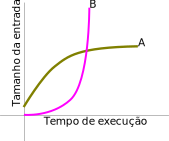
\includegraphics[width=0.5\linewidth]{images/graficoAlgoAeB}
		\caption{Comparação entre algoritmos}
		\label{fig:graficoalgoaeb}
	\end{figure}
	 
\end{frame}




		
	\section{Análise assintótica}
		\begin{frame}
	\frametitle{Análise assintótica}
	\framesubtitle{Limites assintóticos - O que é uma assíntota?}
	\begin{columns}
		\begin{column}{0.5\textwidth}
			\par Dada uma $f(x)=b$ uma assíntota é a curva dada pela equação \ref{eq:assintota}.
			\begin{equation}
				\lim_{x\to\infty} f(x) = b \qquad,
				\label{eq:assintota}
			\end{equation}
		\end{column}
		\begin{column}{0.5\textwidth}
			\begin{figure}
				\centering
				\includegraphics[width=.9\linewidth]{images/assintotas}
				\caption{A função f(x)=1/x tem como assíntotas os eixos coordenados. Fonte: Wikipedia}
				\label{fig:assintotas}
			\end{figure}
		\end{column}
	\end{columns}
\end{frame}

\begin{frame}[fragile]
	\frametitle{Análise assintótica}
	\framesubtitle{Antes começar}
	
	\par Antes de fazer a análise assintótica é necessário aprender a contar o número de instruções primitivas que estão sendo executadas. Geralmente se considera apenas algumas operações elementares como comparações e atribuições.	
\end{frame}

\begin{frame}[fragile]
	\frametitle{Análise assintótica}
	\framesubtitle{Contagem}
	
	\begin{lstlisting}[language=C++, caption={Um algorítimo de tempo constante}, label={lst:umAlgo}]
		
		int valor = 0; 									//Custo 1
		int vetor[] = int[100];					//Custo 1
		for (i=0; i < 100; i++){				// <- 100 vezes
			soma += vetor[i];							//Custo 1
		}
		
		std::cout << soma << std::endl;	//Custo 1
	\end{lstlisting}
	
	
	\begin{lstlisting}[language=C++, caption={Um algorítimo de tempo variável}, label={lst:umAlgo}]
		
		int somatorio(int n, int vetor[]){
			
			int valor = 0; 						//Custo 1
			for (i=0; i < n; i++){		// <- n vezes
				soma += vetor[i];				//Custo 1
			}
			
			return soma;							//Custo 1
		}
	\end{lstlisting}
	
	
\end{frame}

\begin{frame}
	\frametitle{Análise assintótica}
	\framesubtitle{Classes de comportamento assintótico}
	\par Em ordem de tempo crescente:
	\begin{itemize}
		\item $1$ - constante
		\item $\log n$ - logarítimica
		\item $n$ - linear
		\item $n.\log n$ - logarítimica
		\item $n^2$ - quadrática, cúbica, etc. 
		\item $2^n$ - exponencial
		\item $n!$ - fatorial
		\item $n^n$ - vixi...
	\end{itemize}
	\par Ver o exemplo \textit{ordensDeComportamento.ipynb} no jupyter-lab.
\end{frame}

\begin{frame}[fragile]
	\frametitle{Limites assintóticos}
	\framesubtitle{Limites inferiores e superiores}
	\par O limite superior de um algoritmo é o \textbf{maior tempo} que o mesmo leva para executar.
	\par O limite inferior é o \textbf{menor tempo}. 
	\lstinputlisting[language=c++]{codigo/melhorPiorCaso.cpp}
	\par Dependendo do valor do menor elemento o comportamento do algorítimo muda. Testemos o código acima com $vetor = \{1,2,3,4,5\}$ e com $vetor = \{10,5,3,2,-4\}$ e $n = 5$.
\end{frame}

\begin{frame}
	\frametitle{Limites assintóticos}
	\framesubtitle{Limites inferiores e superiores}
	\par \textbf{Melhor Caso}: $1 + 1*n + 1 + 1 + 1 = n + 4$ (linear)
	\par \textbf{Pior Caso}: $1 + 2*n + 1 + 1*n*n + 1 = n2 + 2n + 3$ (quadrático)\newline
	\par A complexidade desse algoritmo pode ser descrita como: $\Omega(n)$ e $O(n^2)$
	\begin{figure}
		\centering
		\includegraphics[width=0.4\linewidth]{images/primeiroOmegaOzao}
		\caption{Gráfico do comportamento do algorítimo}
		\label{fig:primeiroomegaozao}
	\end{figure}
	
\end{frame}

\begin{frame}
	\frametitle{Limites assintóticos}
	\framesubtitle{Limites inferiores e superiores - Exercicios}
	\par Como já foi dito o tempo do algoritmo pode variar segundo a entrada de dados, considerando isto, se faz necessário avalia-lo segundo seu \textbf{melhor} e \textbf{pior} caso de execução.
	
	O melhor caso de execução é aquele que no qual o algoritmo leva menos tempo (executa menos comandos) o pior é aquele que ocupa mais.
\end{frame}

\begin{frame}[fragile]
	\frametitle{Limites assintóticos}
	\framesubtitle{Limites inferiores e superiores - Exercícios}
	\begin{lstlisting}[language=C++,caption={Algoritmo 1}]
		int soma = 0;
		for (int i=0; i<n; i++)
		soma = soma + i;
	\end{lstlisting}
	
	\begin{lstlisting}[language=C++,caption={Algoritmo 2}]
		int soma1 = 0;
		int soma2 = 0;
		for (int i=0; i<n; i++){
			soma1 = soma1 + 1;
			soma2 = soma2 + i;
		}
	\end{lstlisting}
	
\end{frame}

\begin{frame}[fragile]
	\frametitle{Limites assintóticos}
	\framesubtitle{Limites inferiores e superiores - Exercícios}
	
	\begin{lstlisting}[language=C++,caption={Algoritmo 3}]
		int soma1 = 0;
		for (int i=0; i<n; i++){
			soma1 = soma1 + 1;
		}
		for (int j=0; j<n;j++){
			soma1 = soma1 + j;
		}
	\end{lstlisting}
	
	\begin{lstlisting}[language=C++,caption={Algoritmo 4}]
		int soma = 0;
		for (int i=0; i<n; i++){
			for (int j=0; j<m; j++){
				soma = soma + 1;
			}
		}
	\end{lstlisting}
	
\end{frame}

\begin{frame}[fragile]
	\frametitle{Limites assintóticos}
	\framesubtitle{Limites inferiores e superiores - Exercícios}
	
	\begin{lstlisting}[language=C++,caption={Algoritmo 5}]
		int menor = INT_MAX;
		for (int i=0; i<n; i++){
			if (vetor[i] < menor)
			menor = vetor[i];
		}
	\end{lstlisting}
	
\end{frame}

\begin{frame}
	\frametitle{Análise assintótica}
	\framesubtitle{Limites}
	\par Atribui limites superiores, exatos e inferiores para o tempo de execução de um algorítimo expressando os mesmos em forma de funções assintóticas a esse tempo de execução.\newline
	\par Para fazer essa análise usaremos código real e/ou pseudo-código: \textbf{Cuidado com as chamadas informais}.\newline
	
	\par Se assume que o acesso a RAM e as operações primitivas na CPU também tenham um tempo constante.
	\begin{itemize}
		\item o - Limite assintótico superior de ordem superior.
		\item O - Limite assintótico superior.
		\item $\theta$ - Limite assintótico restrito.
		\item $\Omega$ - Limite assintótico inferior.
		\item $\omega$ - Limite assintótico inferior de ordem inferior.
	\end{itemize}
\end{frame}

\begin{frame}
	\frametitle{Limites assintóticos}
	\framesubtitle{Relações entre os comportamentos assintóticos}
	\par Se um algorítimo \textbf{não} é $O$ então também não será $o$
	\par Se o algorítimo é $O$ e $\Omega$ o mesmo não será $\Theta$.
	\par Se o algorítimo é $\Theta$ então não poderá ser $\omega$ ou $o$.
	\par Se o algorítimo é $O$ e \textbf{não} é $\Omega$ então não poderá ser $\Theta$.
	\par Se é $o$ ou $\omega$ então \textbf{não} é $\Theta$. 
\end{frame}

\begin{frame}
	\frametitle{Limites assintóticos}
	\only<1>{
		\framesubtitle{Mas... espera um pouco...}
		\begin{columns}
		\begin{column}{0.8\textwidth}
			\begin{figure}
				\centering
				\includegraphics[width=\linewidth]{images/assintotas2}
				\caption{Assíntotas de $n^2$}
				\label{fig:assintotas2}
			\end{figure}
		\end{column}
		\begin{column}{0.2\textwidth}
			\par Como pode $O(n^2)$ ser o limite assintótico superior se $n^2 \le 6n^2+3n+5$ ?
		\end{column}
		\end{columns}
	}
	\only<2>{
		\framesubtitle{Notação "Ózão" (ou \textit{big O})}
		\par Na notação "Ózão" (ou \textit{big O}) se diz que uma função $f(x)$ domina assintoticamente uma função $g(n)$ quando existem constantes $c$ e $a$ tais que, para \textbf{qualquer} $n \geq a$ é verdadeiro que $c.f(n) \geq g(n)$.\newline
		\par De outra forma podemos dizer que:\newline
		
		\begin{itemize}
			\item $g(n) = O(f(n))$
			\item $g(n)$ é da ordem no máximo $f(n)$
			\item $g(n)$ é $O$ de $f(n)$
			\item $g(n)$ é igual a $O$ de $f(n)$
			\item $g(n)$ pertence a $O$ de $f(n)$
		\end{itemize}
		
		\par Ver o exemplo \textit{ordensDeComportamento.ipynb} no jupyter-lab.
	}
\end{frame}
		
	\section{Análise de algoritmos}
		\begin{frame}
	\frametitle{Tempo de execução \textit{versus} complexidade}
	\par Considerando a tabela abaixo vamos estimar o tempo \textbf{assintótico} de execução doos algoritmos representados.\newline
	
	\begin{center}
		\begin{tabular}{|c|c|c|c|c|c|c|}
			\hline
			\rule[-1ex]{0pt}{2.5ex} Função de custo & \multicolumn{6}{c|}{Tamanho da entrada} \\
			\hline
			\rule[-1ex]{0pt}{2.5ex}  & 10 & 20 & 30 & 40 & 50 & 60 \\
			\hline
			\rule[-1ex]{0pt}{2.5ex} $n.\log n$ & 33 & 43 & 49 & 53 & 56 & 59 \\
			\hline
			\rule[-1ex]{0pt}{2.5ex} $n$ &  &  &  &  &  &  \\
			\hline
			\rule[-1ex]{0pt}{2.5ex} $n^2$ &  &  &  &  &  &  \\
			\hline
			\rule[-1ex]{0pt}{2.5ex} $n^3$ &  &  &  &  &  &  \\
			\hline
			\rule[-1ex]{0pt}{2.5ex} $n^5$ &  &  &  &  &  &  \\
			\hline
			\rule[-1ex]{0pt}{2.5ex} $2^n$ &  &  &  &  &  &  \\
			\hline
			\rule[-1ex]{0pt}{2.5ex} $3^n$ &  &  &  &  &  &  \\
			\hline
			\rule[-1ex]{0pt}{2.5ex} $n!$ &  &  &  &  &  &  \\
			\hline
		\end{tabular}
	\end{center}
\end{frame}

\begin{frame}
	\frametitle{Notação "Ózão" (ou \textit{big O})}
	\only<1>{
		\par Na notação "Ózão" (ou \textit{big O}) se diz que uma função $f(x)$ domina assintoticamente uma função $g(n)$ quando existem constantes $c$ e $a$ tais que, para \textbf{qualquer} $n \geq a$ é verdadeiro que $c.f(n) \geq g(n)$.\newline
		\par De outra forma podemos dizer que:\newline
		
		\begin{itemize}
			\item $g(n) = O(f(n))$
			\item $g(n)$ é da ordem no máximo $f(n)$
			\item $g(n)$ é $O$ de $f(n)$
			\item $g(n)$ é igual a $O$ de $f(n)$
			\item $g(n)$ pertence a $O$ de $f(n)$
			\item o tempo de execução $T(n)$ é $O$
		\end{itemize}
		
		\par Ver o exemplo \textit{ordensDeComportamento.ipynb} no jupyter-lab.
	}
	\only<2>{
		\par Sendo assim se pode dizer, \textbf{por exemplo}, que:
		\begin{itemize}
			\item $n = O(n^2)$
			\item $n^2 = O(n^2)$
			\item $\log{n} = O(n^2)$
			\item $n.\log{n} = O(n^2)$
		\end{itemize}
	
		\par Já que $g(n) \leq c.n^2$ para um certo valor de $c \geq a$.
	}
	\only<3>{
		\par Existe um valor de $c$ para que $n^2+100n = O(n^2)$? \newline
		\par Por exemplo, $c=100$ ou $c=150$ ou $c \geq 100$.
		\begin{equation}
			n^2+100n \leq c.n^2 \Longrightarrow n^2+100n \leq 100.n^2 \Longrightarrow \dfrac{100}{n} \leq 99 \qquad \forall n \geq 2
		\end{equation}
	}
	\only<4>{
		\framesubtitle{Algebra}
		\begin{itemize}
			\item $f(n) = O(f(n))$
			\item $c.O(f(n)) = O(f(n))$, $c = constante$
			\item $O(f(n)) + O(f(n)) = O(f(n))$
			\item $O(O(f(n))) = O(f(n))$
			\item $O(f(n)) + O(g(n)) = O(max(f(n),g(n)))$
			\item $O(f(n)).O(g(n)) = O(f(n).g(n))$
			\item $f(n).O(g(n)) = O(f(n).g(n))$
		\end{itemize}
	}
	\only<5>{
		\framesubtitle{Treinando}
		\begin{enumerate}
			\item $6n^4 + 12n^3 + 12 \qquad$ é $ O(n^4), O(n^5), O(n^6)$?
			\item $3n^2 + 12n.\log{n} \qquad$ é $ O(n^2), O(n^5), O(n)$?
			\item $5n^2 + n.\log{n} + 12 \qquad$ é $ O(n^2), O(n^5)$?
			\item $\log{n} + 4 \qquad $ é $O(\log{n}), O(n)$?
		\end{enumerate}
	}
\end{frame}
\begin{frame}
	\frametitle{Notação Ômega (ou $\Omega$)}
	\only<1>{
		\par Na notação "Ômega" (ou $\Omega$) se diz que uma função $f(x)$ \textbf{é dominada} assintoticamente por uma função $g(n)$ quando existem constantes $c$ e $a$ tais que, para \textbf{qualquer} $n \geq a$ é verdadeiro que $c.f(n) \leq g(n)$.\newline
		\par De outra forma podemos dizer que:\newline
		
		\begin{itemize}
			\item $g(n) = \Omega(f(n))$
			\item $g(n)$ é da ordem no mínimo $f(n)$
			\item $g(n)$ é $\Omega$ de $f(n)$
			\item $g(n)$ é igual a $\Omega$ de $f(n)$
			\item $g(n)$ pertence a $\Omega$ de $f(n)$
			\item o tempo de execução $T(n)$ é $\Omega$
		\end{itemize}
		
		\par Ver o exemplo \textit{ordensDeComportamento.ipynb} no jupyter-lab.
	}
	\only<2>{
		\par Sendo assim se pode dizer, \textbf{por exemplo}, que:
		\begin{itemize}
			\item $n^2 = \Omega(\log{n})$
			\item $n = \Omega(\log{n})$
			\item $n^3 = \Omega(\log{n})$
			\item $n! = \Omega(\log{n})$
		\end{itemize}
		
		\par Já que $g(n) \geq c.\log{n}$ para um certo valor de $c \geq a$.
	}
	\only<3>{
		\framesubtitle{Algebra}
		\begin{itemize}
			\item $f(n) = \Omega(f(n))$
			\item $c.\Omega(f(n)) = \Omega(f(n))$, $c = constante$
			\item $\Omega(f(n)) + \Omega(f(n)) = \Omega(f(n))$
			\item $\Omega(\Omega(f(n))) = \Omega(f(n))$
			\item $\Omega(f(n)) + \Omega(g(n)) = \Omega(max(f(n),g(n)))$
			\item $\Omega(f(n)).\Omega(g(n)) = \Omega(f(n).g(n))$
			\item $f(n).\Omega(g(n)) = \Omega(f(n).g(n))$
		\end{itemize}
	}
	\only<4>{
		\framesubtitle{Observações}
		\par Na prática a notação $\Omega$ não é vista sozinha	em análises de algoritmos, pois é muito otimista.	
	}
\end{frame}

\begin{frame}
	\frametitle{Notação "ozinho" (ou $o$)}
	\only<1>{
		\par Na notação "ozinho" (ou $o$) se diz que uma função $f(x)$ domina assintoticamente uma função $g(n)$ quando existem constantes $c$ e $a$ tais que, para \textbf{qualquer} $n \geq a$ é verdadeiro que $c.f(n) \leq g(n)$, além disso,  $f(n)$ \textbf{é de ordem superior} a $g(n)$.\newline
		\par De outra forma podemos dizer que:\newline
		
		\begin{itemize}
			\item $g(n) = o(f(n))$
			\item $g(n)$ é de ordem menor que $f(n)$
			\item $g(n)$ é $o$ de $f(n)$
			\item $g(n)$ é igual a $o$ de $f(n)$
			\item $g(n)$ pertence a $o$ de $f(n)$
			\item o tempo de execução $T(n)$ é menor que $o$
		\end{itemize}
		
		\par Ver o exemplo \textit{ordensDeComportamento.ipynb} no jupyter-lab.
	}
\end{frame}

\begin{frame}
	\frametitle{Notação "omeguinha" (ou $\omega$)}
	\only<1>{
		\par Na notação "omeguinha" (ou $\omega$) se diz que uma função $f(x)$ \textbf{é dominada} assintoticamente por uma função $g(n)$ quando existem constantes $c$ e $a$ tais que, para \textbf{qualquer} $n \geq a$ é verdadeiro que $c.f(n) \leq g(n)$ , além disso,  $f(n)$ \textbf{é de ordem inferior} a $g(n)$.\newline.
		\par De outra forma podemos dizer que:\newline
		
		\begin{itemize}
			\item $g(n) = \omega(f(n))$
			\item $g(n)$ é de ordem menor que $f(n)$
			\item $g(n)$ é $\omega$ de $f(n)$
			\item $g(n)$ é igual a $\omega$ de $f(n)$
			\item $g(n)$ pertence a $\omega$ de $f(n)$
			\item o tempo de execução $T(n)$ é menor que $\omega$
		\end{itemize}
		
		\par Ver o exemplo \textit{ordensDeComportamento.ipynb} no jupyter-lab.
	}
\end{frame}

\begin{frame}
	\frametitle{Notações $\omega$ e $o$}
	\framesubtitle{Observações}
	\par Na prática a notação $\omega$ é $o$ não são usadas sozinhas (isso quando são vistas) em análises de algoritmos, pois são muito imprecisas.	
\end{frame}

\begin{frame}
	\frametitle{Notação "Theta" (ou $\theta$)}
	\only<1>{
		\par Na notação "Theta" (ou $\theta$) se diz que uma função $f(x)$ \textbf{restringe} a função $g(n)$ quando existem constantes $c_1$, $c_2$ e $a$ tais que, para \textbf{qualquer} $n \geq a$  é verdadeiro que $0 \leq c_1.g(n) \leq f(n) \leq c_2.g(n) \qquad \forall n \geq a$.\newline.
		\par De outra forma podemos dizer que:\newline
		
		\begin{itemize}
			\item $g(n) = \theta(f(n))$
			\item $g(n)$ é de ordem $f(n)$
			\item $g(n)$ é $\theta$ de $f(n)$
			\item $g(n)$ é igual a $\theta$ de $f(n)$
			\item $g(n)$ pertence a $\theta$ de $f(n)$
			\item o tempo de execução $T(n)$ é menor que $\theta$
		\end{itemize}
		
		\par Ver o exemplo \textit{ordensDeComportamento.ipynb} no jupyter-lab.
	}
\end{frame}
		
	\section{Recorrências}
		\begin{frame}
	\frametitle{Recorrências}
	\begin{figure}
		\centering
		\includegraphics[width=1\linewidth]{images/recursivo}
		\caption{}
		\label{fig:recursivo}
	\end{figure}
\end{frame}

\begin{frame}
	\frametitle{Recorrências}
	\par A recorrência é uma forma de descrever o comportamento de algoritmos recursivos.\newline
	\par Para esse tipo de análise usaremos, entre outras coisas, o que se chama de \textbf{relação de recorrência}.
	\par Toda recursão tem um \textbf{caso base} ou \textbf{ponto de parada}. O caso base é o conjunto de instruções que fará com que um valor trivial seja finalmente retornado (ou não) iniciando o desempilhamento da pilha de recursão. Além disso deve existir o \textbf{caso indutivo} ou \textbf{recursão} que é o trecho de código onde a função faz uma chamada a ela mesma empilhando a chamada anterior e suas respectivas variáveis/estados.
	\lstinputlisting[language=C++]{../codigo/algoritmoRecursivo01.cpp}
\end{frame}

\begin{frame}
	\frametitle{Relações de recorrência}
	\framesubtitle{Exemplo 01}
	\par Qual a relação de recorrência desse algoritmo?\\
	\lstinputlisting[language=C++]{../codigo/algoritmoRecursivo01.cpp}
	\par Do \textbf{único} caso indutivo é possível perceber que a entrada é diminuída em \textbf{n-1}, de todo o resto do algoritmo percebe-se que os tempos de execução são constantes, ou seja, $\Theta(1)$.
	\par Então a relação de recorrência é dada por esses valores como colocado na equação \ref{eq:relRecor}. 
	\begin{equation}
		\label{eq:relRecor}
		T(n) = 1.T(n-1) + \Theta(1)
	\end{equation}
\end{frame}

\begin{frame}
	\frametitle{Relações de recorrência}
	\framesubtitle{Exemplo 02}
	\par Qual a relação de recorrência desse algoritmo?\\
	\lstinputlisting[language=C++]{../codigo/algoritmoRecursivo02.cpp}
	\par Dos \textbf{dois} casos indutivos é possível perceber que a entrada é diminuída em \textbf{n-1} e \textbf{n-2}, de todo o resto do algoritmo percebe-se que os tempos de execução são constantes, ou seja, $\Theta(1)$.
	\par Então a relação de recorrência é dada por esses valores como colocado na equação \ref{eq:relRecor01}. 
	\begin{equation}
		\label{eq:relRecor01}
		T(n) = 1.T(n-1) + 1.T(n-2) + \Theta(1)
	\end{equation}
\end{frame}


\begin{frame}
	\frametitle{Relações de recorrência}
	\framesubtitle{Exemplo 03}
	\par Qual a relação de recorrência desse algoritmo?\\
	\lstinputlisting[language=C++]{../codigo/algoritmoRecursivo03.cpp}
	\par Dos \textbf{dois} casos indutivos é possível perceber que a entrada é diminuída em \textbf{n/2} e \textbf{n-2}, de todo o resto do algoritmo percebe-se que os tempos de execução são \textbf{constantes + complexidade n}, ou seja, $\Theta(n)$.
	\par Então a relação de recorrência é dada por esses valores como colocado na equação \ref{eq:relRecor02}. 
	\begin{equation}
		\label{eq:relRecor02}
		T(n) = T(n/2) + T(n/2) + \Theta(n) + \Theta(1) \rightarrow 2.T(n/2) + \Theta(n)
	\end{equation}
\end{frame}

\begin{frame}
	\frametitle{Resolvendo relações de recorrência}
	\begin{itemize}
		\item método da árvore de recursão
		\item método iterativo
		\item método mestre
	\end{itemize}
\end{frame}

\begin{frame}
	\frametitle{Resolvendo relações de recorrência}
	\framesubtitle{Base matemática}
	\begin{columns}
		\begin{column}{0.55\textwidth}
			\begin{equation}
				\begin{aligned} 
					&\sum_{k=1}^{n} a_k = a_1 + a_2 + \dots + a_k\\
					&\sum_{k=1}^{\infty} a_k = \lim\limits_{n \to \infty} \sum_{k=1}^{n} a_k\\
					&\sum_{k=1}^{n} (c.a_k + b_k) = c.\sum_{k=1}^{n} a_k + \sum_{k=1}^{n} b_k\\
					&\sum_{k=1}^{n} \Theta(f(k)) = \Theta\left(	\sum_{k=1}^{n} f(k)\right)
				\end{aligned}
			\end{equation}
		\end{column}
		\begin{column}{0.45\textwidth}
			\begin{equation}
				\begin{aligned}
					&P.A.\\ 
					&a_n = a_1 + (n-1).r\\
					&S_n = \dfrac{n.(a_1 + a_n)}{2}\\
					&P.G.\\
					&a_n = a_1.q^{n-1}\\
					&S_n = \dfrac{a_1.(q^n-1)}{q-1} \qquad &\forall q \geq |1|\\
					&S_n = \dfrac{a_1}{1-q} \qquad &\forall q < |1|
				\end{aligned}
			\end{equation}
		\end{column}
	\end{columns}
\end{frame}

\begin{frame}
	\frametitle{Resolvendo relações de recorrência}
	\framesubtitle{Base matemática}
	\begin{columns}
		\begin{column}{0.5\textwidth}
			\begin{equation}
				\begin{aligned} 
					&\log_ca = k \Leftrightarrow c_k = a\\
					&\log_c(ab) = \log_ca+\log_cb\\
					&\log_ba^n = n.log_ba\\
					&\log_aa=1\\
					&\log n = \lg n = \log_2n\\
					&a = b^{\log_ba}\\
					&a^{\log_bn} = n^{\log_ba}\\
					&\log_ab = \dfrac{\log_cb}{\log_ca}
				\end{aligned}
			\end{equation}
		\end{column}
		\begin{column}{0.5\textwidth}
			\begin{figure}
				\centering
				\includegraphics[width=0.7\linewidth]{images/ogrito}
				\caption{Ahhhhhhh!}
				\label{fig:ogrito}
			\end{figure}
		\end{column}
	\end{columns}
\end{frame}

\begin{frame}
	\frametitle{Resolvendo relações de recorrência - Método da árvore de recursão}
	\framesubtitle{Passos para resolver - Exemplo 0}
		\begin{columns}
		\begin{column}{0.5\textwidth}
			\begin{itemize}
				\item expandir a árvore
				\item calcular a altura \textbf{h}
			\end{itemize}
		
			\par Para entender como expandir a árvore de recursão, ao lado coloquei um exemplo simples para a seguinte relação de recorrência:
			\begin{equation}
				T(n)=T(n-1) + \Theta(1)
			\end{equation}
			\par Ao fazer a expansão se chega no caso-limite em que o tamanho da entrada é igual a 1 ($T(1)$). Dessa forma a altura $\mathbf{h=\Theta(n)}$ já que $h=n-1 \implies \Theta(n)$
		\end{column}
		\begin{column}{0.5\textwidth}
			\begin{figure}
				\centering
				\includegraphics[width=.9\linewidth]{images/arvoreDeRecussao00}
				\caption{Árvore de recursão expandida}
				\label{fig:arvorederecussao00}
			\end{figure}
		\end{column}
	\end{columns}
\end{frame}

\begin{frame}
	\frametitle{Resolvendo relações de recorrência - Método da árvore de recursão}
	\framesubtitle{Passos para resolver - Exemplo 0}
	\begin{columns}
		\begin{column}{0.35\textwidth}
			\begin{itemize}
				\item calcular os custos por nível
				\item somatória dos custos dos níveis \textbf{h} vezes
			\end{itemize}
			\par Nesta fase devemos nos concentrar no \textbf{tempo gasto para combinar os resultados das chamadas recursivas}.\newline
			\par Esse tempo é dado pelo último termo da relação de recorrência.
		\end{column}
		\begin{column}{0.65\textwidth}
			\par Então:
			\begin{equation}
				\begin{aligned}
					&T(n) \to T(n-1) \to T(n-2) \to \dots \to T(n-h) \implies \\
					&\Theta(1) + \Theta(1) + \Theta(1) + \dots + \Theta(1)=\mathbf{\Theta(1)} \implies\\
					&h.\Theta(1) = \Theta(n).\Theta(1) = \mathbf{\Theta(n)}
				\end{aligned}
			\end{equation}
		\end{column}
	\end{columns}
\end{frame}

\begin{frame}
	\frametitle{Resolvendo relações de recorrência - Método da árvore de recursão}
	\framesubtitle{Passos para resolver - Exemplo 1}
	\begin{columns}
		\begin{column}{0.5\textwidth}
			\par Expansão da árvore ao lado.
			\begin{equation}
				T(n)=2T(n/2) + \Theta(n)
			\end{equation}
			\par Analisando a árvore de recursão nota-se que quando a profundidade da árvore atinge seu máximo a altura da mesma é expressa segundo a expressão da equação.
			\begin{equation}
				\begin{aligned}
				&T(n/2^h)=T(1) \implies \\
				&\dfrac{n}{2^h} = 1 \implies \\
				&2^h = n \implies \\
				&\mathbf{h = \log n}
				\end{aligned}
			\end{equation}
		\end{column}
		\begin{column}{0.5\textwidth}
			\begin{figure}
				\centering
				\includegraphics[width=\linewidth]{images/arvoreDeRecusao01}
				\caption{Árvore de recursão expandida}
				\label{fig:arvorederecusao01}
			\end{figure}
		\end{column}
	\end{columns}
\end{frame}


\begin{frame}
	\frametitle{Resolvendo relações de recorrência - Método da árvore de recursão}
	\framesubtitle{Passos para resolver - Exemplo 1}
	\begin{columns}
		\begin{column}{0.35\textwidth}
			\par Nesta fase devemos nos concentrar no \textbf{tempo gasto para combinar os resultados das chamadas recursivas}.\newline
			\par Esse tempo é dado pelo último termo da relação de recorrência.
		\end{column}
		\begin{column}{0.65\textwidth}
			\par Então:
			\begin{equation}
				\begin{aligned}
					&\Theta(n) + \Theta(2.n/2) + \Theta(4.n/4) + \dots + \Theta(2^h . n/2^h) = \\
					&\Theta(n)+\Theta(n)+\Theta(n)+\dots+\Theta(n) = \mathbf{\Theta(n)} \implies \\
					&h . \Theta(n) = \Theta(\log n).\Theta(n) = \mathbf{\Theta(n.\log n)}
				\end{aligned}
			\end{equation}
		\end{column}
	\end{columns}
\end{frame}

\begin{frame}
	\frametitle{Resolvendo relações de recorrência - Método da árvore de recursão}
	\framesubtitle{Exercício 0}
	\par Dadas as relações de recorrência, para cada uma, crie a árvore recursiva expandida e determine o tempo de execução do algoritmo.
	\begin{equation}
		T(n) = 3.T(n/3) + \Theta(n)
	\end{equation}
	\begin{equation}
		T(n) = 2.T(n/2) + \Theta(1)
	\end{equation}
	\begin{equation}
		T(n) = 2.T(n/3) + \Theta(1)
	\end{equation}
\end{frame}

\begin{frame}
	\frametitle{Resolvendo relações de recorrência - Método da árvore de recursão}
	\framesubtitle{Respostas}
	\begin{equation}
		T(n) = \Theta(n.\log n)
	\end{equation}
	\begin{equation}
		T(n) = \Theta(n)
	\end{equation}
	\begin{equation}
		T(n) = \Theta(n^{\log_32})
	\end{equation}
	\par No segundo e terceiros exercícios a dica é notar a progressão geométrica de \textbf{h} termos e razão 2 já que, como já foi dito, é necessário \textbf{somar h vezes} os custos.
\end{frame}

\begin{frame}
	\frametitle{Resolvendo relações de recorrência - Método da árvore de recursão}
	\framesubtitle{Exercício 1}
	\lstinputlisting[language=C++]{../codigo/algoritmoRecursivo.cpp}
	\par Qual a complexidade desse algoritmo?
\end{frame}

\begin{frame}
	\frametitle{Resolvendo relações de recorrência - Método iterativo}
	\par Dada a relação de recorrência
	\begin{equation}
		T(n) \leq T(n/2) + 1
	\end{equation}
	\par Considerando que \textbf{i} indica o número de \textbf{iterações} vamos calcular de forma \textbf{iterativa} o tempo deste algoritmo.
	\begin{equation}
		\label{eq:it1}
		T(n) \leq T(n/2) + 1 \leq T(n/2/2) + 1 + 1 \leq T(n/2/2/2) + 1 + 1 + 1 \leq \mathbf{T(n/2^i) + i} 
	\end{equation}
	\par Sendo assim, para o caso base $T(1)$, note que o tempo do algoritmo \textbf{não} depende de \textbf{i}, portanto, i é tradada como constante.
	\begin{equation}
		T(n/2^i) + i = T(1) \implies T(n/2^i) = T(1) \implies n/2^i = 1 \implies 2^i = n \implies i = \log n
	\end{equation}
	\par Substituindo \textbf{i} no resultado da equação \ref{eq:it1}.
	\begin{equation}
		T(n/2^i) + i \implies T(n/2^{\log n}) + \log n \implies T(1) + \log n \implies T(n) = \mathbf{O(\log n)}
	\end{equation}
	
\end{frame}

\begin{frame}
	\frametitle{Teorema mestre}
	\framesubtitle{Fórmula geral e limitações}
	\par É uma fórmula geral para calcular o tempo de um algoritmo mas tem algumas limitações em relação aos outros métodos já descritos:
	\begin{itemize}
		\item usado para resolver problemas do tipo "dividir para conquistar"
		\item $a =$ é o número de chamadas recursivas simultâneas
		\item $b =$ é a quantidade de subdivisões do problema
		\item $f(n)$ deve ser não negativa
	\end{itemize}
	\par Considerando essas limitações a fórmula é dada na equação \ref{eq:teorMestre}.
	\begin{equation}
		\label{eq:teorMestre}
		T(n) = a.T(n/b) + f(n)
	\end{equation}
\end{frame}

\begin{frame}
	\frametitle{Teorema mestre}
	\framesubtitle{Casos}
	\par Aplicada a fórmula, a avaliação é feita segundo as três condições abaixo:
	\begin{itemize}
		\item $f(n) = O(n^{\log_ba-\epsilon}) \exists \epsilon > 0 \implies T(n) = \Theta(n^{\log_ba})$
		\item $f(n) = \Theta(n^{\log_ba}) \implies T(n) = \Theta(n^{\log_ba}.\log_bn) = \Theta(f(n).\log_bn)$
		\item $f(n) = \Omega(n^{\log_ba+\epsilon})\exists \epsilon>0, a.f(n/b) \leq c.f(n) \forall 0 < c < 1, n=grande \implies T(n) = \Theta(f(n))$
	\end{itemize}
	\par É importante saber que o teorema mestre não necessáriamente descreve o tempo do algoritmo de forma exata: Os resultados obtidos devem ser interpretados como se referindo aos \textbf{casos médios} ou \textbf{piores casos} a depender da estrutura interna do algoritmo (instruções, desvios condicionais, etc.). Leve em consideração a possibilidade de um melhor ou pior caso que resulte em tempos excepcionais. 
\end{frame}

\begin{frame}
	\frametitle{Teorema mestre}
	\framesubtitle{Exercício}
	\par Em quais dos casos abaixo se pode aplicar o teorema mestre?
	\begin{itemize}
		\item $T(n) = 2^n.T(n/2)+n^n$
		\item $T(n) = 0,5.T(n/2)+1/n$
		\item $T(n) = 64.T(n/2) -n^2.\log n$
	\end{itemize}
	\pause
	\par Resposta: \pause \textbf{Nenhum}:
	\par Na primeiro caso o valor $2^n$ não é uma constante inteira, no segundo a mesma coisa, no terceiro $f(n)=-n^2.\log n$
\end{frame}

\begin{frame}
	\frametitle{Teorema mestre}
	\framesubtitle{Exemplo 0}
	\par Vamos resolver a relação de recorrência:
	\begin{equation}
		T(n) = 2.T(n/2) + \Theta(1)
	\end{equation}

	\begin{itemize}
		\item $a = 2$ 
		\item $b = 2$ 
		\item $f(n) = 1 = constante$ 
	\end{itemize}

	\begin{equation}
		1 < n^{\log_ba} \implies 1 < n^{\log_22} \implies 1 < n^1 \implies verdadeiro! \implies T(n)=\Theta(n^{\log_22}) = \mathbf{\Theta(n)}
	\end{equation}
\end{frame}

\begin{frame}
	\frametitle{Teorema mestre}
	\framesubtitle{Exemplo 1}
	\par Vamos resolver a relação de recorrência:
	\begin{equation}
		T(n) = 2.T(n/2) + \Theta(n)
	\end{equation}
	
	\begin{itemize}
		\item $a = 2$ 
		\item $b = 2$ 
		\item $f(n) = n$ 
	\end{itemize}
	
	\begin{equation}
		\begin{aligned}
		&n = n^{\log_ba} \implies \\
		&n = n^{\log_22} \implies \\
		&n = n^1 \implies verdadeiro! \implies \\
		&T(n)=\Theta(f(n).\log_bn) = \mathbf{n.\log n}
		\end{aligned}
	\end{equation}
\end{frame}

\begin{frame}
	\frametitle{Teorema mestre}
	\framesubtitle{Exemplo 2}
	\par Vamos resolver a relação de recorrência:
	\begin{equation}
		T(n) = 2.T(n/2) + \Theta(n^2)
	\end{equation}
	
	\begin{itemize}
		\item $a = 2$ 
		\item $b = 2$ 
		\item $f(n) = n^2$ 
	\end{itemize}
	
	\begin{equation}
		\begin{aligned}
			&n^2 > n^{\log_ba} \implies \\
			&n^2 > n^{\log_22} \implies \\
			&n^2 > n^1 \implies verdadeiro! \implies \\
			&T(n)=\Theta(f(n)) = \mathbf{\Theta(n^2)}
		\end{aligned}
	\end{equation}
\end{frame}

\begin{frame}
	\frametitle{Teorema mestre}
	\framesubtitle{Exercício 0}
	\par Vamos resolver a relação de recorrência:
	\begin{equation}
		\label{eq:tmr00}
		T(n) = 9.T(n/3) + n
	\end{equation}
	\begin{equation}
		\label{eq:tmr01}
		T(n) = 2.T(n/4)+\sqrt{n}
	\end{equation}
	\begin{equation}
		\label{eq:tmr02}
		T(n) = 3.T(n/4)+n.\log n
	\end{equation}
	
\end{frame}

\begin{frame}
	\frametitle{Teorema mestre}
	\framesubtitle{Respostas}
	\only<1>{
		\par Resolvendo a recorrência \ref{eq:tmr00}
		\par Verdadeiro para o primeiro caso:
		\begin{equation}
			\begin{aligned}
				&T(n) = 9.T(n/3) + n \implies\\
				&a=9, b=3, f(n)=n \implies\\
				&f(n) = O(n^{\log_39-\epsilon}) = \\
				&O(n^{2-\epsilon}) \implies\\
				&n \leq c.n^{2-\epsilon}, \epsilon = 1 \therefore\\
				&T(n) = \Theta(n^{\log_ba}) = \\
				&\Theta(n^{\log_39}) = \Theta(n^2)
			\end{aligned}
		\end{equation}
	}
	\only<2>{
		\par Resolvendo a recorrência \ref{eq:tmr01}
		\par Verdadeiro para o segundo caso:
		\begin{equation}
			\begin{aligned}
				&T(n) = 2.T(n/4)+\sqrt{n} \implies\\
				&a=2, b=4, f(n)=\sqrt{n} \implies\\
				&f(n) = \Theta(n^{\log_42}) \implies \\
				&\sqrt{n} = \Theta(n^{0,5}) \implies\\
				&c_1.n^{0,5} \leq \sqrt{n} \leq c_2.n^{0,5}, c_1 = c_2 = 1 \therefore\\
				&T(n) = \Theta(n^{\log_ba}.\log n) = \Theta(n^{\log_42} . \log n) =\\
				&  \Theta(n^{0,5} . \log n) =  \Theta(\sqrt{n} . \log_4 n)
			\end{aligned}
		\end{equation}
	}
	\only<3>{
		\par Resolvendo a recorrência \ref{eq:tmr02}; verdadeiro para o terceiro caso:
		\begin{equation}
			\begin{aligned}
				&T(n) = 3.T(n/4)+n.\log n \implies\\
				&a=3, b=4, f(n)=n.\log n \implies\\
				&f(n) = \Omega(n^{\log_ba + \epsilon}) \implies n.\log n = \Omega(n^{\log_43 + \epsilon}) \implies\\
				&n.\log n = \Omega(n^{0.79 + \epsilon}) \implies n.\log n = \Omega(n^{0.79 + 0,21}), \epsilon = 0,21 \implies \\
				&n.\log n = c.n^1 \implies n.\log n = \Omega(n)! \therefore\\
				&a.f(n/b) \leq c.f(n)? \implies 3.\dfrac{n}{4}.\log\left(\dfrac{n}{4}\right) \leq c.n.\log n \implies \dfrac{3n}{4}.(\log n - \log 4) \leq c.n.\log n \implies \\
				&\dfrac{3n}{4}.(\log n - 2) \leq \dfrac{3n}{4}.\log n, c=\dfrac{3}{4} \implies \log n - 2 \leq \log n \therefore T(n) = \Theta(f(n)) = \Theta(n.\log n).
			\end{aligned}
		\end{equation}
	}
\end{frame}

\begin{frame}
	\frametitle{Tudo em Todo Lugar ao Mesmo Tempo}
	\framesubtitle{Exercício}
	\par Determine a relação de recorrência do algoritmo abaixo para em seguida determinar seu tempo usando o método da \textbf{árvore de recursão}, \textbf{iterativo} e \textbf{mestre}.
	\lstinputlisting[language=C++]{../codigo/algoritmoRecursivo04.cpp}
\end{frame}
		
	\section{Algoritmos de ordenação - baseados em troca}
		\begin{frame}
	\frametitle{Algorítimos de ordenação}
	\framesubtitle{Utilidade}
	\par Analisar algoritmos de ordenação são uma ótima forma de entender e analisar vários outros algoritmos devido a natureza dos problemas, além, é claro, de serem diretamente utilizados em aplicações como banco de dados e localização de padrões.\newline
	
	\par Os algoritmos que teremos contato a partir de agora serão mais complexos de se analisar pois, nem sempre coisas como a relação de recorrência estarão trivialmente definidos.
\end{frame}

\begin{frame}
	\frametitle{Algorítimos de ordenação - baseados em troca}
	\begin{itemize}
		\item \textbf{Burbble-sort} - método do borbulhação
		\item \textbf{Quick-sort} - ordenação por troca de partição
	\end{itemize}
\end{frame}

\begin{frame}
	\frametitle{Algorítimos de ordenação - baseados em troca}
	\framesubtitle{Burbble-sort}
	\par Esse algoritmo percorre várias vezes o vetor de dados a cada iteração comparando cada um de seus elementos com o próximo, sendo que,  se o próximo é menor do que o anterior há uma troca de lugares entre os dois.
	\lstinputlisting[language=C++]{../codigo/burbblesort.cpp}
\end{frame}

\begin{frame}
	\frametitle{Algorítimos de ordenação - baseados em troca}
	\framesubtitle{Exercício 0}
	\par Determine o tempo de execução do \textit{burbble-sort} com seus respectivos melhores e piores tempos se houverem. Use a notação que melhor se encaixa à situação.
	\pause
	\par \textbf{Resposta}: $O(n^2)$.
\end{frame}

\begin{frame}
	\frametitle{Algorítimos de ordenação - baseados em troca}
	\framesubtitle{Quick-sort}
	\par A ideia usada é \textbf{dividir para conquistar}, o vetor é dividido em outros dois menores que são ordenados independentemente para depois serem combinados produzindo assim o resultado final. Tal separação é feita usando-se um \textbf{elemento pivô}, dessa forma, todos os elementos a esquerda do pivô são menores do que ele e todos elementos a direita são maiores que o mesmo
	\par Primeiro passo:
	\begin{itemize}
		\item determinar o elemento pivô: Isso pode ser feito de várias formas, localizar a mediana, fazer uma média entre elementos, etc. 
		\item ordenar os sub-vetores de forma que os elementos a esquerda do pivô são menores que o mesmo e os elementos a direita são maiores.
		\item percorrer simultaneamente o vetor da esquerda para direita, e da direita para esquerda comparando os respectivos elementos e trocando de posição quando necessário.
		\item quando os ponteiros da esquerda e da direita se cruzarem a troca é finalizada.		
	\end{itemize}
\end{frame}

\begin{frame}
	\frametitle{Algorítimos de ordenação - baseados em troca}
	\framesubtitle{Quick-sort}
	
	\par Segundo passo
	\par Ordenar os sub-vetores abaixo e acima do elemento pivô. 
	
	\par Vamos escolher como pivô o elemento $25$.
	
	\par Agora caminhamos com o ponteiro \textbf{menor} para a direita até que encontremos um valor \textbf{maior que o pivô}. 
	
	\par Simultaneamente caminhamos com o ponteiro \textbf{maior} para a esquerda até que encontremos um valor \textbf{menor que o pivô}.\newline
	
	\par $\underset{\underset{menor \rightarrow}{\uparrow}}{\mathbf{25}}, 57, 48, 37, 12, 86, 92, \underset{\underset{\leftarrow maior}{\uparrow}}{\mathbf{33}}$ \newline
	
	\par 25, $\underset{\underset{menor \rightarrow}{\uparrow}}{\mathbf{57}}, 48, 37, \underset{\underset{\leftarrow maior}{\uparrow}}{\mathbf{12}} 86, 92, 33 $
\end{frame}

\begin{frame}
	\frametitle{Algorítimos de ordenação - baseados em troca}
	\framesubtitle{Quick-sort}
	
	\par 25, $\underset{\underset{menor \rightarrow}{\uparrow}}{\mathbf{57}}, 48, 37, \underset{\underset{\leftarrow maior}{\uparrow}}{\mathbf{12}} 86, 92, 33 $\newline
	
	\par Permuta-se os elementos apontados por \textbf{menor} e \textbf{maior}:
	\par 25, $\underset{\underset{menor \rightarrow}{\uparrow}}{\mathbf{12}}, 48, 37, \underset{\underset{\leftarrow maior}{\uparrow}}{\mathbf{57}} 86, 92, 33 $\newline
	
	\par \textbf{Até que} os ponteiros maior e menor \textbf{se cruzem}, assim, o ponteiro \textbf{maior} indica onde se permutar o pivô pelo valor apontado.
	\par 25, $\underset{\underset{\leftarrow maior}{\uparrow}}{\mathbf{12}}$, $\underset{\underset{menor \rightarrow}{\uparrow}}{\mathbf{48}}, 37, 57, 86, 92, 33 $
\end{frame}

\begin{frame}
	\frametitle{Algorítimos de ordenação - baseados em troca}
	\framesubtitle{Quick-sort}
	
	\par \textbf{Até que} os ponteiros maior e menor \textbf{se cruzem}, assim, o ponteiro \textbf{maior} indica onde se permutar o pivô pelo valor apontado.
	\par 25, $\underset{\underset{\leftarrow maior}{\uparrow}}{\mathbf{12}}$, $\underset{\underset{menor \rightarrow}{\uparrow}}{\mathbf{48}}, 37, 57, 86, 92, 33 $\newline
	
	\par 12, $\underset{\underset{\leftarrow maior}{\uparrow}}{\mathbf{25}}$, $\underset{\underset{menor \rightarrow}{\uparrow}}{\mathbf{48}}, 37, 57, 86, 92, 33 $\newline
	
	\par Agora \textbf{divide-se} o vetor em dois pedaços segundo a \textbf{localização do pivô}:
	\par $\underset{\underset{sub-vetor0}{\uparrow}}{\{12\}}$ $\underset{\underset{pivo}{\uparrow}}{(25)}$ $\underset{\underset{sub-vetor1}{\uparrow}}{\{48, 37, 57, 86, 92, 33\}} $\newline
		
	\par Agora reinicia-se o processo \textbf{para cada sub-vetor}, caso um vetor vetor chegue no \textbf{caso base} contendo 1 elemento o consideramos ordenado, no caso de 2 elementos é possivel, usando uma comparação simples, permutar os elementos, se necessário.
\end{frame}

\begin{frame}
	\frametitle{Algorítimos de ordenação - baseados em troca}
	\framesubtitle{Exercício 1}
	\par Implemente o \textit{quick-sort}.
	\par Determine o tempo de execução do \textit{Quick-sort} com seus respectivos melhores e piores tempos se houverem. Use a notação que melhor se encaixa à situação.
	\pause
	\par \textbf{Resposta}: No melhor caso as partiçoes são quebradas ao meio, no pior (vetor ordenado) o pivô quebra o vetor no seu início. $\Omega(n.\log n), O(n^2)$.
	\lstinputlisting[language=C++]{../codigo/quicksort.cpp}
\end{frame}




		
	\section{Algoritmos de ordenação - baseados em inserção}
		\begin{frame}
	\frametitle{Algoritmos de ordenação - baseados em inserção}
	\par Os algoritmos por inserção trabalham de forma análoga a um conjunto de cartas de baralho, essas que são seguradas na mão, a princípio, estão desordenadas, o papel do algoritmo é retirar uma ou mais cartas de suas posições originais e colocar-las na posição correta de forma a configurar uma certa ordem.\newline
	\par $10, 25, 40, 50, \underset{\underset{foraDeOrdem}{\uparrow}}{\mathbf{12}}, 80, 2, 23, \dots $ \newline
	\par $10, \underset{\underset{emOrdem}{\uparrow}}{\mathbf{12}}, 25, 40, 50, 80, 2, 23, \dots $ \newline
	
	\par Perceba que o número $12$ foi \textbf{inserido} entre $10$ e $25$. 
\end{frame}

\begin{frame}
	\frametitle{Algoritmos de ordenação - baseados em inserção}
	\begin{itemize}
		\item \textbf{Inserção simples}
		\item \textbf{Shell-sort}
	\end{itemize}
\end{frame}

\begin{frame}
	\frametitle{Algoritmos de ordenação - baseados em inserção}
	\framesubtitle{Insertion-Sort}
	\par Algoritmo \textbf{Insertion-Sort} segue exatamente a ideia demonstrada no início desta seção, é um algoritmo que retira valores de um local e os coloca em outro deslocando, se necessário, todos os outros elementos do vetor. 
	\lstinputlisting[language=C++]{../codigo/insercaoSimples.cpp}
\end{frame}

\begin{frame}
	\frametitle{Algoritmos de ordenação - baseados em inserção}
	\framesubtitle{Exercício 0}
	\par Determine o tempo de execução do \textit{algoritmo de inserção simples} com seus respectivos melhores e piores tempos se houverem. Use a notação que melhor se encaixa à situação.
	\pause
	\par \textbf{Resposta}:
	\par $\Omega(n)$ para o vetor ordenado, $O(n^2)$ para o vetor ordenado de forma decrescente.
\end{frame}

\begin{frame}
	\frametitle{Algoritmos de ordenação - baseados em inserção}
	\framesubtitle{Shell-Sort}
	\par O Shell-Sort é uma evolução do algoritmo anterior, avaliando a inserção simples nota-se que o melhor caso é quando o vetor já está ordenado, sendo assim, o Shell-Sort adota a estratégia de \textbf{dividir para conquistar} subdividindo o vetor em vários pares de valores usando "saltos" que vão diminuindo em quantidade com o tempo de forma que fica cada vez mais \textbf{provável} que o vetor já esteja ordenado, diminuindo assim o tempo total de execução.\newline
	\par No exemplo abaixo, mostro um exemplo com passo $k=5$:

	\par $
	\apontar{par0}{\textcolor{blue}{55}}, 
	\apontar{par1}{\textcolor{yellow}{33}}, 
	\apontar{par2}{\textcolor{red}{12}},  
	\apontar{par3}{\textcolor{gray}{01}}, 
	\apontar{par0}{\textcolor{blue}{19}}, 
	\apontar{par1}{\textcolor{yellow}{10}},
	\apontar{par2}{\textcolor{red}{70}}, 
	\apontar{par3}{\textcolor{gray}{25}} 
	$
\end{frame}

\begin{frame}
	\frametitle{Algoritmos de ordenação - baseados em inserção}
	\framesubtitle{Shell-Sort}
	\par $
	\apontar{par0}{\textcolor{blue}{55}}, 
	\apontar{par1}{\textcolor{yellow}{33}}, 
	\apontar{par2}{\textcolor{red}{12}},  
	\apontar{par3}{\textcolor{gray}{01}}, 
	\apontar{par0}{\textcolor{blue}{19}}, 
	\apontar{par1}{\textcolor{yellow}{10}},
	\apontar{par2}{\textcolor{red}{70}}, 
	\apontar{par3}{\textcolor{gray}{25}}
	$ \newline
	\par $
	\apontar{par0}{\textcolor{blue}{19}}, 
	\apontar{par1}{\textcolor{yellow}{10}}, 
	\apontar{par2}{\textcolor{red}{12}},  
	\apontar{par3}{\textcolor{gray}{01}}, 
	\apontar{par0}{\textcolor{blue}{55}}, 
	\apontar{par1}{\textcolor{yellow}{33}},
	\apontar{par2}{\textcolor{red}{70}}, 
	\apontar{par3}{\textcolor{gray}{25}}
	\leftarrow $ Primeira passada $k=5$ \newline
	\pause
	\par $
	\apontar{par0}{\textcolor{blue}{19}}, 
	\apontar{par1}{\textcolor{yellow}{10}}, 
	\apontar{par2}{\textcolor{red}{12}},  
	\apontar{par0}{\textcolor{blue}{01}}, 
	\apontar{par1}{\textcolor{yellow}{55}}, 
	\apontar{par2}{\textcolor{red}{33}},
	\apontar{par0}{\textcolor{blue}{70}}, 
	\apontar{par1}{\textcolor{yellow}{25}}
	$ \newline
	
	\par $
	\apontar{par0}{\textcolor{blue}{01}}, 
	\apontar{par1}{\textcolor{yellow}{10}}, 
	\apontar{par2}{\textcolor{red}{12}},  
	\apontar{par0}{\textcolor{blue}{19}}, 
	\apontar{par1}{\textcolor{yellow}{25}}, 
	\apontar{par2}{\textcolor{red}{33}},
	\apontar{par0}{\textcolor{blue}{70}}, 
	\apontar{par1}{\textcolor{yellow}{55}}
	\leftarrow$ Segunda passada $k=4$ \newline
	\pause
	\par $
	\apontar{par0}{\textcolor{blue}{01}}, 
	\apontar{par1}{\textcolor{yellow}{10}}, 
	\apontar{par0}{\textcolor{blue}{12}},  
	\apontar{par1}{\textcolor{yellow}{19}}, 
	\apontar{par0}{\textcolor{blue}{25}}, 
	\apontar{par1}{\textcolor{yellow}{33}},
	\apontar{par0}{\textcolor{blue}{70}}, 
	\apontar{par1}{\textcolor{yellow}{55}}
	$ \newline
	
	\par $
	\apontar{par0}{\textcolor{blue}{01}}, 
	\apontar{par1}{\textcolor{yellow}{10}}, 
	\apontar{par0}{\textcolor{blue}{12}},  
	\apontar{par1}{\textcolor{yellow}{19}}, 
	\apontar{par0}{\textcolor{blue}{25}}, 
	\apontar{par1}{\textcolor{yellow}{33}},
	\apontar{par0}{\textcolor{blue}{70}}, 
	\apontar{par1}{\textcolor{yellow}{55}}
	\leftarrow$ Terceira passada $k=2$
\end{frame}

\begin{frame}
	\frametitle{Algoritmos de ordenação - baseados em inserção}
	\framesubtitle{Shell-Sort}
	
	\par Quando $k=1$ (1 partição = todo o vetor) aplica-se então o algoritmo de inserção simples! 
	\lstinputlisting[language=C++]{../codigo/shellSort.cpp}
\end{frame}

\begin{frame}
	\frametitle{Algoritmos de ordenação - baseados em inserção}
	\framesubtitle{Pesquisa}
	\par Determine o tempo de execução do \textit{Shell-Sort} com seus respectivos melhores e piores tempos se houverem. Use a notação que melhor se encaixa à situação. Como o tamanho das partições muda o tempo do algoritmo? \textbf{Indique as referências}.
\end{frame}

		

	\section{Algoritmos de ordenação - baseados em seleção}
		\begin{frame}
	\frametitle{Algoritmos de ordenação - baseados em seleção}
	\par A ideia é selecionar um elemento e já colocá-lo em sua posição correta definitiva evitando assim futuras permutações com o mesmo.
\end{frame}

\begin{frame}
	\frametitle{Algoritmos de ordenação - baseados em seleção}
	\begin{itemize}
		\item \textbf{Selection-Sort}
		\item \textbf{Heap-Sort}
	\end{itemize}
\end{frame}

\begin{frame}
	\frametitle{Algoritmos de ordenação - baseados em seleção}
	\framesubtitle{Selection-sort}
	\par É um algoritmo que seleciona o menor elemento do vetor e o coloca no início do mesmo, em seguida, seleciona o menor elemento do \textbf{vetor n-1} e o coloca no início desse vetor resultante. Esse algoritmo se repete até que o vetor esteja totalmente ordenado. 
	
	\par $55,33,12,01,19,10,70,25$	
	\par $\underbrace{55,33,12,\apontar{menor}{01},19,10,70,25}$
	\pause
	\par $\underbrace{\apontar{menor}{01},55,33,12,55,19,10,70,25}$
	\pause
	\par $01,\underbrace{55,33,12,55,19,\apontar{menor}{10},70,25}$
	\pause
	\par $01,\underbrace{\apontar{menor}{10},33,12,55,19,55,70,25}$
\end{frame}

\begin{frame}
	\frametitle{Algoritmos de ordenação - baseados em seleção}
	\framesubtitle{Selection-sort}
		\begin{columns}
		\begin{column}{0.5\textwidth}
			\par $01,\underbrace{\apontar{menor}{10},33,12,55,19,55,70,25}$
			\pause
			\par $01, 10, \underbrace{33,\apontar{menor}{12},55,19,55,70,25}$
			\pause
			\par $01, 10, \underbrace{\apontar{menor}{12},33,55,19,55,70,25}$
			\pause
			\par $01, 10, 12,\underbrace{33,55,\apontar{menor}{19},55,70,25}$
			\pause
			\par $01, 10, 12,\underbrace{\apontar{menor}{19},55,33,55,70,25}$
		\end{column}
		\begin{column}{0.5\textwidth}
			\par $01, 10, 12, 19,\underbrace{55,33,55,70,\apontar{menor}{25}}$
			\pause
			\par $01, 10, 12, 19,\underbrace{\apontar{menor}{25},33,55,70,55}$
			\pause
			\par $01, 10, 12, 19, 25, \underbrace{\apontar{menor}{33},55,70,55}$
			\pause
			\par $01, 10, 12, 19, 25, 33,\underbrace{\apontar{menor}{55},70,55}$
			\pause
			\par $01, 10, 12, 19, 25, 33, 55, \underbrace{70, \apontar{menor}{55}}$
			\pause
			\par $01, 10, 12, 19, 25, 33, 55, 55, 70 \leftarrow$ ordenado!
		\end{column}
	\end{columns}
\end{frame}

\begin{frame}
	\frametitle{Algoritmos de ordenação - baseados em seleção}
	\framesubtitle{Selection-sort - Exercício 0}
	\par Algoritmo:
	\lstinputlisting[language=C++]{../codigo/selectionSort.cpp}

	\par Determine o tempo de execução do \textit{Selection-sort} com seus respectivos melhores e piores tempos se houverem. Use a notação que melhor se encaixa à situação.
	\pause
	\par \textbf{Resposta:}
	\par $\Theta(n^2)$

\end{frame}

\begin{frame}
	\frametitle{Algoritmos de ordenação - baseados em seleção}
	\framesubtitle{Heap-sort}
	\par São algoritmos baseados em uma estrutura dados chamada de \textbf{Heap} que nada mais é do que um tipo de \textbf{árvore binária} de dados. É uma evolução do \textit{selection-sort}, no nosso caso vai trazer sempre em seu elemento raíz o maior valor do vetor (\textit{heap máximo}) e será balanceado a esquerda.
	\par Pode ser implementado de várias formas mas, como o objetivo aqui é ordenar um vetor, tal implementação não passará disso, portanto a árvore binária que representa esta estrutura de dados terá como nós filhos as expressões \ref{eq:fe} e \ref{eq:fd} e como nó pai \ref{eq:np}.
	\begin{equation}
		\label{eq:fe}
		filhoEsquerdo(k)=2k+1
	\end{equation}
	\begin{equation}
		\label{eq:fd}
		filhoDireito(k)=2k+2
	\end{equation}
	\begin{equation}
		\label{eq:np}
		pai(k)=\dfrac{k-1}{2}
	\end{equation}
\end{frame}
	
\begin{frame}
	\frametitle{Algoritmos de ordenação - baseados em seleção}
	\framesubtitle{Heap-sort}
	\par Decerto o ajuste do \textit{Heap} tem seu custo, no entanto, devido ao balanceamento da árvore tal custo é de ordem (descubra isso no exercício).
	\par Por fim, eis a definição do \textit{heap-sort}:
	\begin{itemize}
		\item construir o \textit{heap} máximo
		\item trocar a raiz (o maior elemento cuja localização é 0) com o elemento da última posição do vetor.
		\item diminuir o tamanho do \textit{heap} em 1
		\item rearranjar o \textit{heap} máximo se necessário
		\item repetir o processo n-1 vezes
	\end{itemize}
\end{frame}

\begin{frame}
	\frametitle{Algoritmos de ordenação - baseados em seleção}
	\framesubtitle{Heap-sort}
	\tikzset{
		heap/.style={
			every node/.style={circle,draw},
			level 1/.style={sibling distance=30mm},
			level 2/.style={sibling distance=15mm},
			level 3/.style={sibling distance=10mm},
			level 4/.style={sibling distance=5mm}
		},
		fontbf/.style={font=\bfseries}
	}
	\only<1>{
	\begin{columns}
		\begin{column}{0.5\textwidth}
			\begin{tikzpicture}[heap]
				\node {16}
				child{
					node{14}
					child{
						node{08}
						child{
							node{02}
						}
						child{
							node{04}
						}
					}
					child{
						node{07}
						child{
							node{01}
						}
					}
				}
				child{
					node{10}
					child{
						node{09}
					}
					child{
						node{03}
					}
				};
			\end{tikzpicture}
		\end{column}
		\begin{column}{0.5\textwidth}
			\par $
			\apontar{0}{16}, 
			\apontar{1}{14}, 
			\apontar{2}{10},  
			\apontar{3}{08}, 
			\apontar{4}{07}, 
			\apontar{5}{09},
			\apontar{6}{03}, 
			\apontar{7}{02},
			\apontar{8}{04}, 
			\apontar{9}{01}
			$
		\end{column}
	\end{columns}
}
	\only<2>{
	\begin{columns}
		\begin{column}{0.5\textwidth}
			\begin{tikzpicture}[heap, fontbf]
				\node{\textcolor{green}{16}}
				child{
					node{14}
					child{
						node{08}
						child{
							node{02}
						}
						child{
							node{04}
						}
					}
					child{
						node{07}
						child{
							node{\textcolor{green}{01}}
						}
					}
				}
				child{
					node{10}
					child{
						node{09}
					}
					child{
						node{03}
					}
				};
			\end{tikzpicture}
		\end{column}
		\begin{column}{0.5\textwidth}
			\par $
			\apontar{0}{\textcolor{green}{16}}, 
			\apontar{1}{14}, 
			\apontar{2}{10},  
			\apontar{3}{08}, 
			\apontar{4}{07}, 
			\apontar{5}{09},
			\apontar{6}{03}, 
			\apontar{7}{02},
			\apontar{8}{04}, 
			\apontar{9}{\textcolor{green}{01}}
			$
		\end{column}
	\end{columns}
}
\only<3>{
	\begin{columns}
		\begin{column}{0.5\textwidth}
			\begin{tikzpicture}[heap, fontbf]
				\node{\textcolor{green}{01}}
				child{
					node{14}
					child{
						node{08}
						child{
							node{02}
						}
						child{
							node{04}
						}
					}
					child{
						node{07}
						child{
							node{\textcolor{gray}{16}}
						}
					}
				}
				child{
					node{10}
					child{
						node{09}
					}
					child{
						node{03}
					}
				};
			\end{tikzpicture}
		\end{column}
		\begin{column}{0.5\textwidth}
			\par $
			\apontar{0}{\textcolor{green}{01}}, 
			\apontar{1}{14}, 
			\apontar{2}{10},  
			\apontar{3}{08}, 
			\apontar{4}{07}, 
			\apontar{5}{09},
			\apontar{6}{03}, 
			\apontar{7}{02},
			\apontar{8}{04}, 
			\apontar{9}{\textcolor{gray}{16}}
			$
		\end{column}
	\end{columns}
}
\only<4>{
	\par Ajustando o \textit{heap}
	\begin{columns}
		\begin{column}{0.5\textwidth}
			\begin{tikzpicture}[heap, fontbf]
				\node{14}
				child{
					node{01}
					child{
						node{08}
						child{
							node{02}
						}
						child{
							node{04}
						}
					}
					child{
						node{07}
					}
				}
				child{
					node{10}
					child{
						node{09}
					}
					child{
						node{03}
					}
				};
			\end{tikzpicture}
		\end{column}
		\begin{column}{0.5\textwidth}
			\par $
			\apontar{0}{14}, 
			\apontar{1}{01}, 
			\apontar{2}{10},  
			\apontar{3}{08}, 
			\apontar{4}{07}, 
			\apontar{5}{09},
			\apontar{6}{03}, 
			\apontar{7}{02},
			\apontar{8}{04}, 
			\apontar{9}{\textcolor{gray}{16}}
			$
		\end{column}
	\end{columns}
}
\only<5>{
	\par Ajustando o \textit{heap}
	\begin{columns}
		\begin{column}{0.5\textwidth}
			\begin{tikzpicture}[heap, fontbf]
				\node{14}
				child{
					node{08}
					child{
						node{01}
						child{
							node{02}
						}
						child{
							node{04}
						}
					}
					child{
						node{07}
					}
				}
				child{
					node{10}
					child{
						node{09}
					}
					child{
						node{03}
					}
				};
			\end{tikzpicture}
		\end{column}
		\begin{column}{0.5\textwidth}
			\par $
			\apontar{0}{14}, 
			\apontar{1}{08}, 
			\apontar{2}{10},  
			\apontar{3}{01}, 
			\apontar{4}{07}, 
			\apontar{5}{09},
			\apontar{6}{03}, 
			\apontar{7}{02},
			\apontar{8}{04}, 
			\apontar{9}{\textcolor{gray}{16}}
			$
		\end{column}
	\end{columns}
}
\only<6>{
	\par \textit{heap} ajustado!
	\begin{columns}
		\begin{column}{0.5\textwidth}
			\begin{tikzpicture}[heap, fontbf]
				\node{14}
				child{
					node{08}
					child{
						node{04}
						child{
							node{02}
						}
						child{
							node{01}
						}
					}
					child{
						node{07}
					}
				}
				child{
					node{10}
					child{
						node{09}
					}
					child{
						node{03}
					}
				};
			\end{tikzpicture}
		\end{column}
		\begin{column}{0.5\textwidth}
			\par $
			\apontar{0}{14}, 
			\apontar{1}{08}, 
			\apontar{2}{10},  
			\apontar{3}{04}, 
			\apontar{4}{07}, 
			\apontar{5}{09},
			\apontar{6}{03}, 
			\apontar{7}{02},
			\apontar{8}{01}, 
			\apontar{9}{\textcolor{gray}{16}}
			$
			\par Agora é só repetir o processo!
		\end{column}
	\end{columns}
}
\end{frame}

\begin{frame}
	\frametitle{Algoritmos de ordenação - baseados em seleção}
	\framesubtitle{Heap-sort - Exercício 0}

	\only<1>{
		\par Implemente o \textit{heap-sort}.
		\par Determine o tempo de execução para o \textbf{ajuste do heap máximo}, em seguida, descubra o tempo total de execução do \textit{heap-sort} com seus respectivos melhores e piores tempos se houverem. Use a notação que melhor se encaixa à situação.
	}
	\only<2>{
		\par \textbf{Resposta}:
		Ajuste do heap máximo: $\Theta(\log n)$, tempo do algoritmo: $O(n.\log n)$.
		\lstinputlisting[language=C++]{../codigo/heapsort.cpp}
	}
\end{frame}

\begin{frame}
	\frametitle{Algoritmos de ordenação - baseados em seleção}
	\framesubtitle{Merge-sort}
	\par  Merge-sort também usa uma estratégia de "dividir  para conquistar" até o momento em que cada elemento do vetor esteja com um par ou sozinho (caso base), a partir desse momento, os elementos são comparados dois a dois no que se chama “etapa de intercalação” , essa etapa, remonta o vetor de forma que o mesmo fique ordenado.
	\par $\apontar{vetor}{\underbrace{10,02,50,52,07,34,03,01,39,00}}$
	\par $\apontar{vetor/2}{\underbrace{10,02,50,52,07}},\apontar{vetor/2}{\underbrace{34,03,01,39,00}}$
	\par $\apontar{vetor/4}{\underbrace{10,02}},\apontar{vetor/4}{\underbrace{50,52,07}},\apontar{vetor/4}{\underbrace{34,03}},\apontar{vetor/4}{\underbrace{01,39,00}}$
	\par $\apontar{vetor/8}{\underbrace{10}},\apontar{vetor/8}{\underbrace{02}},\apontar{vetor/8}{\underbrace{50}},\apontar{vetor/8}{\underbrace{52,07}},\apontar{vetor/8}{\underbrace{34}},\apontar{vetor/8}{\underbrace{03}},\apontar{vetor/8}{\underbrace{01}},\apontar{vetor/8}{\underbrace{39,00}}$
\end{frame}

\begin{frame}
	\frametitle{Algoritmos de ordenação - baseados em seleção}
	\framesubtitle{Merge-sort}
	\par $\apontar{vetor/8}{\underbrace{10}},\apontar{vetor/8}{\underbrace{02}},\apontar{vetor/8}{\underbrace{50}},\apontar{vetor/8}{\underbrace{52,07}},\apontar{vetor/8}{\underbrace{34}},\apontar{vetor/8}{\underbrace{03}},\apontar{vetor/8}{\underbrace{01}},\apontar{vetor/8}{\underbrace{39,00}}$
	\par $\apontar{vetor/4}{\underbrace{02,10}},\apontar{vetor/4}{\underbrace{07,50,52}},\apontar{vetor/4}{\underbrace{03,34}},\apontar{vetor/4}{\underbrace{00,01,39}}$
	\par $\apontar{vetor/2}{\underbrace{02,07,10,50,52}},\apontar{vetor/2}{\underbrace{00,01,03,34,39}}$
	\par $\apontar{vetor}{\underbrace{00,01,02,03,07,10,34,39,50,52}}$
\end{frame}

\begin{frame}
	\frametitle{Algoritmos de ordenação - baseados em seleção}
	\framesubtitle{Merge-Sort}
	\lstinputlisting[language=C++]{../codigo/mergesort.cpp}
\end{frame}

\begin{frame}
	\frametitle{Algoritmos de ordenação - baseados em seleção}
	\framesubtitle{Merge-Sort}
	\lstinputlisting[language=C++]{../codigo/mergesort2.cpp}
\end{frame}

\begin{frame}
	\frametitle{Algoritmos de ordenação - baseados em seleção}
	\framesubtitle{Merge-sort - Exercício 0}
	
	\par Determine o tempo de execução do \textit{Merge-sort} com seus respectivos melhores e piores tempos se houverem. Use a notação que melhor se encaixa à situação.
	\pause
	\par \textbf{Resposta:}
	\par Com a relação de recorrência $T(n)=2T(n/2) + n$ e pelo teorema mestre temos:
	\par $O(n.\log n)$
\end{frame}





		
	\section{Algoritmos de busca}
		\begin{frame}
	\frametitle{Algoritmos de busca}
	\par Agora que conhecemos uma boa parte dos métodos de ordenação é possível mergulhar nos algoritmos de busca, esses que são extensamente usados em aplicações como bancos de dados ou qualquer outra aplicação em que seja necessário encontrar alguma informação.
\end{frame}

\begin{frame}
	\frametitle{Algoritmos de busca}
	\framesubtitle{Busca linear}
	\par Algoritmo simples: Itere sobre o vetor comparando item-a-item com o valor procurado. Se encontrar retorne sua posição, do contrário retorne -1.
\end{frame}

\begin{frame}
	\frametitle{Algoritmos de busca}
	\framesubtitle{Busca binária}
	\par A busca binária, para que funcione bem, tem como requerimento um vetor ordenado representado como uma \textbf{grafo}, posto isso, o algoritmo recursivamente vai dividindo o vetor ao meio até que o item central seja o que está sendo procurado.
\end{frame}

\begin{frame}
	\frametitle{Algoritmos de busca}
	\framesubtitle{Busca binária - Exercício 0}
	\par Implemente a busca binária.
	\pause
	\par \textbf{Resposta:}
	\lstinputlisting[language=C++]{../codigo/algoritmoRecursivo04.cpp}
\end{frame}


		
	\section{Algoritmos baseados em grafos}
		\begin{frame}
	\frametitle{Algoritmos baseados em grafos}
	\par Essa estrutura pode ajudar na resolução e modelagem de vários problemas como o de ordenação como já foi vista com o \textit{heap-sort}, de busca como na \textit{árvore binária}, modelagem de mapas, relacionamentos em redes de pessoas ou computadores, etc.
	\par Os relacionamentos podem ser de:
	\begin{itemize}
		\item conexão ( o que se conecta com o que )
		\item precedência ( o que vem antes do que )
		\item exclusão mutua ( como as coisas se agrupam? elas tem ligação? )
		\item prefêrência ( o que se encaixa melhor e onde )
	\end{itemize}
\end{frame}

\begin{frame}
	\frametitle{Algoritmos baseados em grafos}
	\par Grafos $G$ são estruturas que representam relacionamentos par-a-par entre pontos ou objetos. Os pontos são os \textbf{vértices ou nós} e as \textbf{arestas} (ou arcos quando são direcionais) são os relacionamentos. \textbf{Neste material}, ao conjunto dos vértices daremos o nome de $V(G)$ e ao conjunto das arestas nomearemos como $A(G)$.
	\begin{columns}
		\begin{column}{0.3\textwidth}
			\begin{figure}
				\centering
				
\includegraphics[width=0.9\linewidth]{images/grafoGenerico}
				\caption{Um grafo}
				\label{fig:grafogenerico}
			\end{figure}
		\end{column}
		\begin{column}{0.7\textwidth}
			\begin{itemize}
				\item se $\{a,b,c,d,e,f,g,h,i\}$ são vértices de um grafo então $G = \{a,b,c,d,e,f,g,h,i\}$
				\item se $a = uv / u \in G, v \in G \therefore  a = aresta \in A(G)$ então:
				\begin{itemize}
					\item $u, v$ são adjacentes
					\item $u, v$ são extremos de $a$
					\item $a$ passa por $uv$ e $a$ é delimitada por $u, v$
				\end{itemize}
				\item Se $u \in V(G)$ o grau de $u$ é a quantidade de vizinhos $d_G(u)$
				\item o grau mínimo é $\delta(G)$ e o máximo é $\Delta(G)$
				 \item $\sum_{v \in V(G)} d_G(v) = 2.|A(G)|$, ou seja, a soma dos graus é igual a duas vezes o total de arestas 
			\end{itemize}
		\end{column}
	\end{columns}
\end{frame}

\begin{frame}
	\frametitle{Algoritmos baseados em grafos}
	\framesubtitle{Grafos simples}
	\begin{itemize}
		\item não tem arestas paralelas (duas arestas ligando o mesmo par de vértices)
		\item laços (um vértice ligado a ele mesmo)
	\end{itemize}
\end{frame}

\begin{frame}
	\frametitle{Algoritmos baseados em grafos}
	\framesubtitle{Digrafos}
	\begin{columns}
	\begin{column}{0.5\textwidth}
		\par Quando a lista dos vértices não é suficiente para representar  as relações entre os mesmos e essas dependem de uma \textbf{procedência} se pode usar os digrafos como representação de tal situação. Um digrafo é um conjunto de dois outros conjuntos onde o primeiro representa os vértices e o segundo contém \textbf{pares ordenados} indicando as relações de precedência.
		
		\begin{equation}
			\begin{aligned}	
				D=	
				\begin{cases}
					V(G) = \{a,b,c,d,e,f,g\} \\
					A(G) = \{ab,bg,ce,de,fg\}
				\end{cases}
			\end{aligned}
		\end{equation}

	\end{column}
	\begin{column}{0.5\textwidth}
			\par Se $ a = uv $ é um \textbf{arco} de $D$ então:
			\begin{itemize}
				\item $u$ é cabeça e $v$ é a cauda
				\item $a$ sai de $u$ e vai para $v$
				\item o grau de entrada $d^-_D(u)$ de $u$ é a qtde de arcos que entram em $u$
				\item o grau de saída $d^+_D(u)$ de $u$ é a qtde de arcos que saem de $u$
				\item a vizinhança de entrada de $u$ é o conjunto de todos os vértices que entram em $u$, $N^-_D(u)$
				\item a vizinhança de saída de $u$ é o conjunto de todos os vértices que saem de $u$, $N^+_D(u)$
			\end{itemize}
		\end{column}
	\end{columns}
\end{frame}

\begin{frame}
	\frametitle{Algoritmos baseados em grafos}
	\framesubtitle{Digrafos}
	\par Para qualquer digrafo $D$ vale:
	\begin{itemize}
		\item $ \sum_{v \in V(D)} d_D^+(v) = \sum_{v \in V(D)} d_D^-(v) = |A(D)| $, ou seja, a soma total de todos os graus de saída é igual a soma de todos os graus de entrada que é igual ao número total de arcos.
		\item Todo digrafo pode gerar um grafo subjacente que nada mais é do que um grafo sem suas direções.
		\item Todo grafo pode ser a base de construção de um \textbf{digrafo associado} $D(G)$ adicionando-se \textbf{arcos paralelos} a cada par de vértices. Ao digrafo que não usa arcos paralelos chamaremos de \textbf{digrafo orientado} $\overrightarrow{G}$.
		\item Os arcos podem ter associados a eles valores $w(uv)$ que serão chamados de \textbf{pesos}.
	\end{itemize}
\end{frame}

\begin{frame}
	\frametitle{Algoritmos baseados em grafos}
	\framesubtitle{Digrafos}
	\par No entanto, na maioria das vezes, representaremos grafos e digrafos da mesma forma pois, mesmo que não haja relações de precedência entre os nós, é preciso indicar as arestas de tal grafo. 
\end{frame}

\begin{frame}
	\frametitle{Algoritmos baseados em grafos}
	\framesubtitle{Representações}
	\par Como já foi visto um grafo pode ser representado por um vetor simples desde que o algoritmo que o trata seja projetado devidamente para usar esta estrutura. No entanto, nem sempre é prático, possível ou eficiente usar uma estrutura tão simples, portanto temos que usar outros tipos:
	\begin{itemize}
		\item lista de adjacências: São listas que, dado um vértice, contém uma \textbf{lista ligada} que contêm todos os vizinhos daquele nó ou, no caso dos digrafos todos os nós de saída daquele vértice.
		\item matrizes de adjacências: É uma \textbf{matriz quadrada} de dimensão igual a quantidade de vértices do grafo na qual a linha $u$ que se cruza com a coluna $v$ indicam se tais vértices são adjacentes.
	\end{itemize}
\end{frame}

\begin{frame}
	\frametitle{Algoritmos baseados em grafos}
	\framesubtitle{Representações: Lista de adjacências}
	\begin{columns}
	\begin{column}{0.6\textwidth}
		\begin{figure}
			\centering
			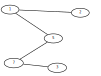
\includegraphics[width=0.4\linewidth]{images/listasDeAdjacencias}
			\caption{Ponteiros em rosa, lista ligada em verde}
			\label{fig:listasdeadjacencias}
		\end{figure}
		\par Memória ocupada: $V(G)$ ponteiros + $2.A(G)$ itens de lista ligada =  $\Theta(V(G) + A(G))$
		\par Tempo de busca por adjacências: $\Omega(1), O(n)$
		\par Bom para grafos esparsos com poucas arestas pois, se $V(G) = n \implies A(G) = \dfrac{n.(n+1)}{2} \implies O(n^2)$ de memória.
	\end{column}
	\begin{column}{0.4\textwidth}
		\begin{figure}
			\centering
			\includegraphics[width=\linewidth]{images/listasDeAdjacenciasGrafo}
			\caption{Exemplo de grafo}
			\label{fig:listasdeadjacenciasgrafo}
		\end{figure}
	\end{column}
\end{columns}
\end{frame}

\begin{frame}
	\frametitle{Algoritmos baseados em grafos}
	\framesubtitle{Representações: Matriz de adjacências}
	\begin{columns}
		\begin{column}{0.4\textwidth}
		\begin{figure}
			\centering
			\includegraphics[width=\linewidth]{images/listasDeAdjacenciasGrafo}
			\caption{Exemplo de grafo}
			\label{fig:listasdeadjacenciasgrafo2}
		\end{figure}
		\end{column}
		\begin{column}{0.6\textwidth}
			\begin{equation}
				\left[
				\begin{matrix}
					& \mathbf{a}&\mathbf{b}&\mathbf{c}&\mathbf{d}&\mathbf{e} \\
					\mathbf{a}& 0&1&1&1&0 \\
					\mathbf{b}& 1&0&0&0&0 \\
					\mathbf{c}& 1&0&0&0&1 \\
					\mathbf{d}& 1&0&0&0&1 \\
					\mathbf{e}& 0&0&1&1&0 \\
				\end{matrix}
				\right]
			\end{equation}
			
			\par Na matriz as arestas $ab$, $bc$ e $dc$ são representadas.\newline
			\par Memória ocupada: $\Theta(n^2)$ para todos os casos.
			\par Tempo de busca por adjacências: $\Theta(1)$
			\par Melhor para grafos muito densos.
		\end{column}
	\end{columns}
\end{frame}

\begin{frame}
	\frametitle{Algoritmos baseados em grafos}
	\framesubtitle{Exercício 0}
	\par Represente os conjuntos do grafo abaixo, informe o grau de cada nó, represente a matriz de adjacências e a lista de adjacências.
		\begin{columns}
		\begin{column}{0.6\textwidth}
			\begin{figure}
				\centering
				\includegraphics[width=.8\linewidth]{images/listasDeAdjacenciasGrafo2}
				\caption{Outro exemplo de grafo}
				\label{fig:listasdeadjacenciasgrafo3}
			\end{figure}
		\end{column}
		\pause
		\begin{column}{0.4\textwidth}
			\par \textbf{Resposta}:
			\only<2>{
				\par $ V(G)  = \{a,b,c,d,e,f\} $
				\par $ A(G)  = \{ab,ac,ad,de,df,ce,fd,fb\} $
				\par $ d_G(a) = 3 $
				\par $ d_G(b) = 2 $
				\par $ d_G(d) = 3 $
				\par $ d_G(c) = 2 $
				\par $ d_G(e) = 2 $
				\par $ d_G(f) = 2 $
			}
			\only<3>{
			\begin{equation}
				\left[
				\begin{matrix}
					& \mathbf{a}&\mathbf{b}&\mathbf{c}&\mathbf{d}&\mathbf{e}&\mathbf{f} \\
					\mathbf{a}& 0&1&1&1&0&0 \\
					\mathbf{b}& 1&0&0&0&0&1 \\
					\mathbf{c}& 1&0&0&0&1&0 \\
					\mathbf{d}& 1&0&0&0&1&1 \\
					\mathbf{e}& 0&0&1&1&0&0 \\
					\mathbf{f}& 0&1&0&1&0&0
				\end{matrix}
				\right]
			\end{equation}
			}
			\only<4>{
				\par $ a \rightarrow b \rightarrow c \rightarrow d $
				\par $ b \rightarrow a \rightarrow f $
				\par $ c \rightarrow a  \rightarrow e $
				\par $ d \rightarrow e  \rightarrow f $
				\par $ e \rightarrow d \rightarrow c $
				\par $ f \rightarrow d  \rightarrow b $
			}
		\end{column}
	\end{columns} 
\end{frame}

\begin{frame}[allowframebreaks]
	\frametitle{Algoritmos baseados em grafos}
	\framesubtitle{Exemplo de lista de adjacências}
	\lstinputlisting[language=C++]{../codigo/listaDeAdjacencia.cpp}
\end{frame}


\begin{frame}
	\frametitle{Algoritmos baseados em grafos}
	\framesubtitle{Exercício 1}
	\par \textbf{Programe} em c ou c++ a \textbf{matriz de adjacências} e adicione os nós como representado abaixo:
	\begin{figure}
		\centering
		\includegraphics[width=.5\linewidth]{images/listasDeAdjacenciasGrafoExercicio}
		\caption{Outro exemplo de grafo}
		\label{fig:listasdeadjacenciasgrafo4}
	\end{figure}
\end{frame}

\begin{frame}
	\frametitle{Algoritmos baseados em grafos}
	\framesubtitle{Removendo vértices}
	\begin{columns}
		\begin{column}{0.4\textwidth}
			\par Até agora vimos como construir e como consultar algumas informações de um grafo mas e se precisarmos \textbf{remover} algum nó?
		\end{column}
		\begin{column}{0.6\textwidth}
			\begin{figure}
				\centering
				\includegraphics[width=0.8\linewidth]{images/remocaoDeVertice00}
				\caption{Remoção de vértice}
				\label{fig:remocaodevertice00}
			\end{figure}
		\end{column}
	\end{columns}
\end{frame}

\begin{frame}
	\frametitle{Algoritmos baseados em grafos}
	\framesubtitle{Removendo vértices - Matriz de adjacências}
	\begin{columns}
		\begin{column}{0.4\textwidth}
			\only<1>{
				\begin{equation}
					\left[
					\begin{matrix}
						 & \mathbf{1}&\mathbf{2}&\mathbf{3}&\mathbf{4}&\mathbf{5}&\mathbf{6}&\mathbf{7} \\
						\mathbf{1}& 0&1&0&0&1&0&0 \\
						\mathbf{2}& 1&0&0&1&0&0&0 \\
						\mathbf{3}& 0&0&0&1&0&0&1 \\
						\mathbf{4}& 0&1&1&0&1&0&0 \\
						\mathbf{5}& 1&0&0&1&0&0&1 \\
						\mathbf{6}& 0&0&0&0&0&0&0 \\
						\mathbf{7}& 0&0&1&0&1&0&0
					\end{matrix}
					\right]
				\end{equation}
				\par Basta essa representação para excluir um nó???
			}
			\only<2>{
				\begin{equation}
					\left[
					\begin{matrix}
						 & \mathbf{1}&\mathbf{2}&\mathbf{3}&\mathbf{\textcolor{green}{4}}&\mathbf{5}&\mathbf{6}&\mathbf{7} \\
						\mathbf{1}& 0&1&0&\textcolor{green}{0}&1&0&0 \\
						\mathbf{2}& 1&0&0&\textcolor{green}{0}&0&0&0 \\
						\mathbf{3}& 0&0&0&\textcolor{green}{0}&0&0&1 \\
						\mathbf{\textcolor{green}{4}}& \textcolor{green}{0}&\textcolor{green}{0}&\textcolor{green}{0}&\textcolor{green}{0}&\textcolor{green}{0}&\textcolor{green}{0}&\textcolor{green}{0} \\
						\mathbf{5}& 1&0&0&\textcolor{green}{0}&0&0&1 \\
						\mathbf{6}& 0&0&0&\textcolor{green}{0}&0&0&0 \\
						\mathbf{7}& 0&0&1&\textcolor{green}{0}&1&0&0
					\end{matrix}
					\right]
				\end{equation}
				\par Não! O nó continua existindo mas, sem ligação alguma.
			}
			\only<3>{
				\begin{equation}
					\left[
					\begin{matrix}
						 & \mathbf{1}&\mathbf{2}&\mathbf{3}&\mathbf{\textcolor{green}{4}}&\mathbf{5}&\mathbf{6}&\mathbf{7} \\
						\mathbf{1}& 0&1&0&\textcolor{green}{-1}&1&0&0 \\
						\mathbf{2}& 1&0&0&\textcolor{green}{-1}&0&0&0 \\
						\mathbf{3}& 0&0&0&\textcolor{green}{-1}&0&0&1 \\
						\mathbf{\textcolor{green}{4}}& \textcolor{green}{-1}&\textcolor{green}{-1}&\textcolor{green}{-1}&\textcolor{green}{-1}&\textcolor{green}{-1}&\textcolor{green}{-1}&\textcolor{green}{-1} \\
						\mathbf{5}& 1&0&0&\textcolor{green}{-1}&0&0&1 \\
						\mathbf{6}& 0&0&0&\textcolor{green}{-1}&0&0&0 \\
						\mathbf{7}& 0&0&1&\textcolor{green}{-1}&1&0&0
					\end{matrix}
					\right]
				\end{equation}
				\par Porém podemos introduzir um terceiro símbolo que dá conta do recado!
			}
		\end{column}
		\begin{column}{0.6\textwidth}
			\only<1>{
				\begin{figure}
					\centering
					\includegraphics[width=0.8\linewidth]{images/remocaoDeVertice00}
					\caption{Remoção de vértice}
					\label{fig:remocaodevertice01}
				\end{figure}
			}
			\only<2>{
				\begin{figure}
					\centering
					\includegraphics[width=0.8\linewidth]{images/remocaoDeVertice01}
					\caption{Remoção de vértice}
					\label{fig:remocaodevertice02}
				\end{figure}
			}
			\only<3>{
				\begin{figure}
					\centering
					\includegraphics[width=0.8\linewidth]{images/remocaoDeVertice02}
					\caption{Remoção de vértice}
					\label{fig:remocaodevertice03}
				\end{figure}
			}
		\end{column}
	\end{columns}
\end{frame}

\begin{frame}
	\frametitle{Algoritmos baseados em grafos}
	\framesubtitle{Exercício 2}
	\par \textbf{Implemente} em c ou c++ a \textbf{remoção de nós} e a \textbf{remoção de arestas}
\end{frame}

\begin{frame}
	\frametitle{Algoritmos baseados em grafos}
	\framesubtitle{Subgrafos}
	\par Considere:
	\begin{equation}
		\begin{aligned}
			\begin{cases}
				&V(G) = \{a,b,c,d,e,f\} \\
				&A(G) = \{ab,ac,ad,dc,ef,fa,be\}
			\end{cases}
		\end{aligned}
	\end{equation}
	\par Então:
	\par Seja $u$ e $v$ dois vértices, um conjunto $H$ é subgrafo de $G$ se $V(H) \subseteq V(G), A(H) \subseteq A(G) / (u,v) \in V(H)$
	\par Um subgrafo $H$ é \textbf{gerador} se $H \subseteq G, V(H) = V(G)$
	\par Se $S \subseteq V(G), G[S]$ é o grafo induzido por $S$
	\par Se $F \subseteq A(G), G[S]$ é o grafo induzido por $F$\newline
	\par É importante notar que os subgrafos mantém as relações definidas anteriormente entre seus vértices.
\end{frame}

\begin{frame}
	\frametitle{Algoritmos baseados em grafos}
	\framesubtitle{Passeios}
	\par Passeios são operações cuja finalidade é visitar os vértices de um grafo, tal procedimento só é possível se houverem arestas entre os vértices visitados.
		\begin{equation}
		\begin{aligned}
			\begin{cases}
				&V(G) = \{a,b,c,d,e,f\} \\
				&A(G) = \{ab,ac,ad,dc,ef,fa,be\}
			\end{cases}
		\end{aligned}
	\end{equation}
	\par considerando o grafo acima \textbf{um dos} passeios possíveis é: 
	\par $P_1=\{a,b,e,f,a,c\}$
	\par O comprimento do passeio é dado pela \textbf{quantidade de vértices do mesmo}.
	\par Passeios fechados começam e terminam no mesmo vértice.
	\par Passeios abertos começam e terminam em vértices distintos. 
\end{frame}

\begin{frame}
	\frametitle{Algoritmos baseados em grafos}
	\framesubtitle{Passeios}
	\par Passeios que \textbf{não repetem} vértices são chamados de \textbf{caminhos}. Caminhos com $n$ vértices são chamados de $P_n$: $P_1, P_5, etc.$
	\par Passeios que \textbf{não repetem} vértices \textbf{exceto os extremos} são chamados de \textbf{ciclo}. Ciclos com $n$ vértices são chamados de $C_n$
	\par Passeios geram subgrafos.
	\par Grafos completos são aqueles nos quais existem arestas entre todos os vértices. Grafos completos com $n$ vértices são chamados de $K_n$: $A(K_n) = \dfrac{n(n-1)}{2}$
	\par $G$ é conexo se \textbf{todos} os pares de vértices são conectados por arestas.
	\par Em \textbf{digrafos} pode \textbf{ou não} ser verdade que $C_n =\{a, b, c, d\} \implies C_n^{'} =\{d, c, b, a\}$
	\par Em um \textbf{digrafo} se houverem caminhos entre quaisquer vértices $a \rightarrow b$ e $b \rightarrow a$ então esse digrafo é \textbf{fortemente conexo}.
\end{frame}

\begin{frame}
	\frametitle{Algoritmos baseados em grafos}
	\framesubtitle{Exercício 03}
	\par Crie exemplos que mostrem \textbf{todas} as propriedades dos \textbf{digrafos, grafos e seus respectivos subgrafos e passeios}.
\end{frame}

\begin{frame}
	\frametitle{Algoritmos baseados em grafos}
	\framesubtitle{Distâncias entre digrafos}
	\par A distância ($dist_G(u,v)$) entre dois vértices em um digrafo é dada pela quantidade de arestas de um vértice até o outro, se estes vértices não estiverem conectados então se diz que a distância é infinita ($\infty$).
	\par Lembre-se que a distância em grafos e digrafos pode variar sensivelmente.
	\par Em grafos e digrafos cujas arestas tem \textbf{pesos} a distância ($dist^w_G(u,v)$) é dada pelo \textbf{menor} valor da soma das arestas (menor distância).
\end{frame}

\begin{frame}
	\frametitle{Algoritmos baseados em grafos}
	\framesubtitle{O problema do caminho mínimo}
	\par O caminho mínimo é aquele que tem o menor valor de soma das arestas, atualmente esse problema só é possivel de se resolver se:
	\begin{itemize}
		\item o grafo não tem aresta com peso negativo
		\item o digrafo não tem um ciclo com peso negativo
	\end{itemize}
\end{frame}

\begin{frame}
	\frametitle{Algoritmos baseados em grafos}
	\framesubtitle{Exercício 04}
	\par Crie um algoritmo que calcula a distância mínima entre dois vértices.
	\par Qual o tempo de execução assintótico?
	\par Esse tempo é bom? Justifique.
\end{frame}

\begin{frame}
	\frametitle{Algoritmos de busca em grafos}
	\framesubtitle{Árvores}
	\par 
	Como já vimos anteriormente no algoritmo \textit{heap-sort} as vezes é necessário a implementação (seja na lógica ou em uma estrutura) de uma árvore mas, o que é uma isso? Assim como na natureza a árvore representa uma estrutura hierárquica na qual algumas partes se ligam a \textbf{uma} outra parte de forma recursiva formando assim uma estrutura parecida com que se pode chamar de fractal de linhas e nós. No contexto dos algoritmos de busca árvores são extremamente úteis pois, geralmente, diminuem muito o tempo para localização de um valor.
	
	\tikzset{
		tree/.style={
			every node/.style={rectangle,draw},
			level 1/.style={sibling distance=40mm},
			level 2/.style={sibling distance=20mm},
			level 3/.style={sibling distance=10mm},
		},
		fontbf/.style={font=\bfseries}
	}
	\begin{figure}
		\begin{tikzpicture}[tree]
			\node {20}
			child{
				node{10}
				child{node{5}}
				child{node{7}}
			}
			child{
				node{11}
				child{node{1}}
				child{node{2}}
			};
		\end{tikzpicture}
	\end{figure}
\end{frame}

\begin{frame}
	\frametitle{Algoritmos de busca em grafos}
	\framesubtitle{Árvores}
	
	\tikzset{
		tree/.style={
			every node/.style={rectangle,draw},
			level 1/.style={sibling distance=40mm},
			level 2/.style={sibling distance=20mm},
			level 3/.style={sibling distance=10mm},
		},
		fontbf/.style={font=\bfseries}
	}
	\begin{figure}
		\begin{tikzpicture}[tree]
			\node {20}
			child{
				node{10}
				child{node{5}}
				child{node{7}}
			}
			child{
				node{11}
				child{node{1}}
				child{node{2}}
			};
		\end{tikzpicture}
	\end{figure}
	\par Considerando que um grafo é dito \textbf{conexo} se existir \textbf{pelo menos um caminho entre cada par de vértices} do grafo. Se pode dizer que uma árvore é um \textbf{grafo conexo} que \textbf{não contêm ciclos} e, por consequência, cujo o número de arestas é o número de vértices - 1.
\end{frame}

\begin{frame}
	\frametitle{Algoritmos de busca em grafos}
	\framesubtitle{Árvores - Exercício 05}
	\par Dê exemplos de grafos que não são árvores.
\end{frame}

\begin{frame}
	\frametitle{Algoritmos de busca em grafos}
	\framesubtitle{Árvores - Propriedades}
	\par Se o grafo $G$ representa uma árvore ($T$) então \textbf{é equivalente} dizer que:
	\begin{itemize}
		\item existe um único caminho entre os dois vértices de $G$
		\item $G$ é conexo para toda aresta pertencente a $G$ $(a \in A(G))$ e remover um aresta o torna desconexo.
		\item é um \textbf{grafo conexo} que \textbf{não contêm ciclos} e, por consequência, cujo o número de arestas é o número de vértices - 1
		\item se $G$ não tem ciclos então todo par de vértices \textbf{não adjacentes} formará um ciclo caso se trace um aresta entre os mesmos.
	\end{itemize}
\end{frame}

\begin{frame}
	\frametitle{Algoritmos de busca em grafos}
	\framesubtitle{Árvores - Propriedades}
	\par Se o grafo $G$ representa uma árvore então:
	\begin{itemize}
		\item Se $uv \notin A(T), uv \in V(T)$ então adicionar esta aresta cria um \textbf{ciclo}.
		\item Se $\forall c \in A(T)$ formam ciclos então suas deleções criam uma árvore.
		\item Se $T \subseteq G$ e $T$ é uma árvore e $V(T) = V(G)$ então $G$ é conexo e $V(T) = V(G)$ é \textbf{geradora}.
		\item Criar um aresta entre um vértice que \textbf{não} pertence a árvore e outro que pertence mantém a árvore já que não cria ciclos.
		\item Em \textbf{digrafos} árvores se chamam \textbf{arvorecências} sendo que todo vértice deve ter grau de entrada = 1 \textbf{exceto o vértice raíz}.
	\end{itemize}
\end{frame}

\begin{frame}
	\frametitle{Algoritmos de busca em grafos}
	\framesubtitle{Árvores - Busca em largura - BFS}
	\par Dado um grafo não árvore, é possível, a partir dele, construir uma árvore usando o algoritmo de busca em largura, encontrar algum vértice ou ainda determinar se um grafo é conexo ou não.
\end{frame}

\begin{frame}
	\frametitle{Algoritmos de busca em grafos}
	\framesubtitle{Árvores - Busca em largura}
	\par Dado o grafo abaixo vamos fazer a busca em largura do mesmo.
	\begin{figure}
		\centering
		\includegraphics[width=0.75\linewidth]{images/buscaEmLargura00}
		\caption{}
		\label{fig:buscaemlargura00}
	\end{figure}
\end{frame}

\begin{frame}
	\frametitle{Algoritmos baseados em grafos}
	\framesubtitle{Árvores - Busca em largura - BFS}
	\setlength{\tabcolsep}{0.5em}
	\begin{tabular}{|c|c|c|c|c|c|c|c|c|c|c|c|c|c|c|c|c|c|c|c|c|}
		\hline
		\rule[0ex]{0pt}{0ex}&1&2&3&4&5&6&7&8&9&10&11&12&13&14&15&16&17&18&19&20 \\
		\hline
		\rule[0ex]{0pt}{0ex}V&0&0&0&0&0&0&0&0&0&0&0&0&0&0&0&0&0&0&0&0 \\
		\hline
		\rule[0ex]{0pt}{0ex}A&0&0&0&0&0&0&0&0&0&0&0&0&0&0&0&0&0&0&0&0 \\
		\hline
	\end{tabular}
	\par $F:\{\}$
	\begin{columns}
		\begin{column}{0.5\textwidth}
			\begin{figure}
				\centering
				\includegraphics[width=\linewidth]{images/buscaEmLargura00}
				\caption{Grafo}
				\label{fig:buscaemlargura01}
			\end{figure}
		\end{column}
		\begin{column}{0.5\textwidth}
			\par Esse algoritmo começa com a criação de uma estrutura que marca quais vértices foram visitados ($V$), quais seus respectivos predecessores ($A$) e uma fila ($F$).
			\par Em seguida se escolhe de forma arbitrária um vértice por onde começar. Comecemos pelo vértice $2$, sendo assim, o mesmo entra na fila.
		\end{column}
	\end{columns}
\end{frame}

\begin{frame}
	\frametitle{Algoritmos baseados em grafos}
	\framesubtitle{Árvores - Busca em largura - BFS}
	\setlength{\tabcolsep}{0.5em}
	\begin{tabular}{|c|c|c|c|c|c|c|c|c|c|c|c|c|c|c|c|c|c|c|c|c|}
		\hline
		\rule[0ex]{0pt}{0ex}&1&2&3&4&5&6&7&8&9&10&11&12&13&14&15&16&17&18&19&20 \\
		\hline
		\rule[0ex]{0pt}{0ex}V&0&0&0&0&0&0&0&0&0&0&0&0&0&0&0&0&0&0&0&0 \\
		\hline
		\rule[0ex]{0pt}{0ex}A&2& &2&2&0&0&0&0&0&0&2&0&0&0&0&0&0&0&0&0 \\
		\hline
	\end{tabular}
	\par $F:\{\cancel{2},4,3,1,11\}$
	\begin{columns}
		\begin{column}{0.5\textwidth}
			\begin{figure}
				\centering
				\includegraphics[width=\linewidth]{images/buscaEmLargura01}
				\caption{Grafo}
				\label{fig:buscaemlargura02}
			\end{figure}
		\end{column}
		\begin{column}{0.5\textwidth}
			\par Agora removemos o item mais antigo da fila e depois adicionamos na mesma seus vizinhos.
			\par Em seguida marcamos os nós visitados e indicamos seu predecessor (que é o $2$).
		\end{column}
	\end{columns}
\end{frame}

\begin{frame}
	\frametitle{Algoritmos baseados em grafos}
	\framesubtitle{Árvores - Busca em largura - BFS}
	\setlength{\tabcolsep}{0.5em}
	\begin{tabular}{|c|c|c|c|c|c|c|c|c|c|c|c|c|c|c|c|c|c|c|c|c|}
		\hline
		\rule[0ex]{0pt}{0ex}&1&2&3&4&5&6&7&8&9&10&11&12&13&14&15&16&17&18&19&20 \\
		\hline
		\rule[0ex]{0pt}{0ex}V&1&1&1&1&0&0&1&1&0&0&1&0&0&0&0&0&0&0&0&0 \\
		\hline
		\rule[0ex]{0pt}{0ex}A&2& &2&2&0&0&4&4&0&0&2&0&0&0&0&0&0&0&0&0 \\
		\hline
	\end{tabular}
	\par $F:\{\cancel{2},\cancel{4},3,1,11,7,8\}$
	\begin{columns}
		\begin{column}{0.5\textwidth}
			\begin{figure}
				\centering
				\includegraphics[width=\linewidth]{images/buscaEmLargura02}
				\caption{Grafo}
				\label{fig:buscaemlargura03}
			\end{figure}
		\end{column}
		\begin{column}{0.5\textwidth}
			\par Então \textbf{novamente} removemos o item mais antigo da fila e depois adicionamos na mesma seus vizinhos.
			\par Em seguida marcamos os nós visitados e indicamos seu predecessor (que é o $4$).
			\par Se faz isso \textbf{até que não exista item algum na fila}
		\end{column}
	\end{columns}
\end{frame}

\begin{frame}
	\frametitle{Algoritmos baseados em grafos}
	\framesubtitle{Árvores - Busca em largura - BFS}
	\setlength{\tabcolsep}{0.5em}
	\begin{tabular}{|c|c|c|c|c|c|c|c|c|c|c|c|c|c|c|c|c|c|c|c|c|}
		\hline
		\rule[0ex]{0pt}{0ex}&1&2&3&4&5&6&7&8&9&10&11&12&13&14&15&16&17&18&19&20 \\
		\hline
		\rule[0ex]{0pt}{0ex}V&1&1&1&1&1&0&1&1&0&0&1&0&0&0&0&0&0&0&0&0 \\
		\hline
		\rule[0ex]{0pt}{0ex}A&2& &2&2&3&0&4&4&0&0&2&0&0&0&0&0&0&0&0&0 \\
		\hline
	\end{tabular}
	\begin{columns}
		\begin{column}{0.5\textwidth}
			\only<1>{
				\par $F:\{\cancel{2},\cancel{4},\cancel{3},1,11,7,8,5\}$
				\begin{figure}
					\centering
					\includegraphics[width=\linewidth]{images/buscaEmLargura03}
					\caption{Grafo}
					\label{fig:buscaemlargura04}
				\end{figure}
			}
			\only<2>{
				\par $F:\{\cancel{2},\cancel{4},\cancel{3},\cancel{1},11,7,8,5\}$
				\begin{figure}
					\centering
					\includegraphics[width=\linewidth]{images/buscaEmLargura04}
					\caption{Grafo}
					\label{fig:buscaemlargura05}
				\end{figure}
			}
		\end{column}
		\begin{column}{0.5\textwidth}

		\end{column}
	\end{columns}
\end{frame}

\begin{frame}
	\frametitle{Algoritmos baseados em grafos}
	\framesubtitle{Árvores - Busca em largura - BFS}
	\setlength{\tabcolsep}{0.5em}
	\begin{tabular}{|c|c|c|c|c|c|c|c|c|c|c|c|c|c|c|c|c|c|c|c|c|}
		\hline
		\rule[0ex]{0pt}{0ex}&1&2&3&4&5&6&7&8&9&10&11&12&13&14&15&16&17&18&19&20 \\
		\hline
		\rule[0ex]{0pt}{0ex}V&1&1&1&1&1&0&1&1&1&1&1&0&0&0&0&0&0&0&0&0 \\
		\hline
		\rule[0ex]{0pt}{0ex}A&2& &2&2&3&0&4&4&11&11&2&0&0&0&0&0&0&0&0&0 \\
		\hline
	\end{tabular}
	\begin{columns}
		\begin{column}{0.5\textwidth}
			\only<1>{
				\par $F:\{\cancel{2},\cancel{4},\cancel{3},\cancel{1},\cancel{11},\cancel{7},8,5,10,9\}$
				\begin{figure}
					\centering
					\includegraphics[width=\linewidth]{images/buscaEmLargura05}
					\caption{Grafo}
					\label{fig:buscaemlargura06}
				\end{figure}
			}
			\only<2>{
				\par $F:\{\cancel{2},\cancel{4},\cancel{3},\cancel{1},\cancel{11},\cancel{7},8,5,10,9\}$
				\begin{figure}
					\centering
					\includegraphics[width=\linewidth]{images/buscaEmLargura06}
					\caption{Grafo}
					\label{fig:buscaemlargura07}
				\end{figure}
			}
		\end{column}
		\begin{column}{0.5\textwidth}

		\end{column}
	\end{columns}
\end{frame}

\begin{frame}
	\frametitle{Algoritmos baseados em grafos}
	\framesubtitle{Árvores - Busca em largura - BFS}
	\setlength{\tabcolsep}{0.5em}
	\begin{tabular}{|c|c|c|c|c|c|c|c|c|c|c|c|c|c|c|c|c|c|c|c|c|}
		\hline
		\rule[0ex]{0pt}{0ex}&1&2&3&4&5&6&7&8&9&10&11&12&13&14&15&16&17&18&19&20 \\
		\hline
		\rule[0ex]{0pt}{0ex}V&1&1&1&1&1&1&1&1&1&1&1&0&0&0&0&0&0&0&0&0 \\
		\hline
		\rule[0ex]{0pt}{0ex}A&2& &2&2&3&5&4&4&11&11&2&0&0&0&0&0&0&0&0&0 \\
		\hline
	\end{tabular}
	\begin{columns}
		\begin{column}{0.5\textwidth}
			\only<1>{
				\par $F:\{\cancel{2},\cancel{4},\cancel{3},\cancel{1},\cancel{11},\cancel{7},\cancel{8},5,10,9\}$
				\begin{figure}
					\centering
					\includegraphics[width=\linewidth]{images/buscaEmLargura07}
					\caption{Grafo}
					\label{fig:buscaemlargura08}
				\end{figure}
			}
			\only<2>{
				\par $F:\{\cancel{2},\cancel{4},\cancel{3},\cancel{1},\cancel{11},\cancel{7},\cancel{8},\cancel{5},10,9,6\}$
				\begin{figure}
					\centering
					\includegraphics[width=\linewidth]{images/buscaEmLargura08}
					\caption{Grafo}
					\label{fig:buscaemlargura09}
				\end{figure}
			}
		\end{column}
		\begin{column}{0.5\textwidth}

		\end{column}
	\end{columns}
\end{frame}

\begin{frame}
	\frametitle{Algoritmos baseados em grafos}
	\framesubtitle{Árvores - Busca em largura - BFS}
	\setlength{\tabcolsep}{0.5em}
	\begin{tabular}{|c|c|c|c|c|c|c|c|c|c|c|c|c|c|c|c|c|c|c|c|c|}
		\hline
		\rule[0ex]{0pt}{0ex}&1&2&3&4&5&6&7&8&9&10&11&12&13&14&15&16&17&18&19&20 \\
		\hline
		\rule[0ex]{0pt}{0ex}V&1&1&1&1&1&1&1&1&1&1&1&0&0&0&0&0&0&0&0&0 \\
		\hline
		\rule[0ex]{0pt}{0ex}A&2& &2&2&3&5&4&4&11&11&2&0&0&0&0&0&0&0&0&0 \\
		\hline
	\end{tabular}
	\begin{columns}
		\begin{column}{0.5\textwidth}
			\only<1>{
				\par $F:\{\cancel{2},\cancel{4},\cancel{3},\cancel{1},\cancel{11},\cancel{7},\cancel{8},\cancel{5},\cancel{10},9,6\}$
				\begin{figure}
					\centering
					\includegraphics[width=\linewidth]{images/buscaEmLargura09}
					\caption{Grafo}
					\label{fig:buscaemlargura10}
				\end{figure}
			}
			\only<2>{
				\par
	$F:\{\cancel{2},\cancel{4},\cancel{3},\cancel{1},\cancel{11},\cancel{7},\cancel{8},\cancel{5},\cancel{10},\cancel{9},6\}$
				\begin{figure}
					\centering
					\includegraphics[width=\linewidth]{images/buscaEmLargura10}
					\caption{Grafo}
					\label{fig:buscaemlargura11}
				\end{figure}
			}
		\end{column}
		\begin{column}{0.5\textwidth}

		\end{column}
	\end{columns}
\end{frame}

\begin{frame}
	\frametitle{Algoritmos baseados em grafos}
	\framesubtitle{Árvores - Busca em largura - BFS}
	\setlength{\tabcolsep}{0.5em}
	\begin{tabular}{|c|c|c|c|c|c|c|c|c|c|c|c|c|c|c|c|c|c|c|c|c|}
		\hline
		\rule[0ex]{0pt}{0ex}&1&2&3&4&5&6&7&8&9&10&11&12&13&14&15&16&17&18&19&20 \\
		\hline
		\rule[0ex]{0pt}{0ex}V&1&1&1&1&1&1&1&1&1&1&1&0&0&0&0&0&0&0&0&0 \\
		\hline
		\rule[0ex]{0pt}{0ex}A&2& &2&2&3&5&4&4&11&11&2&0&0&0&0&0&0&0&0&0 \\
		\hline
	\end{tabular}
	\begin{columns}
		\begin{column}{0.5\textwidth}
			\par $F:\{\cancel{2},\cancel{4},\cancel{3},\cancel{1},\cancel{11},\cancel{7},\cancel{8},\cancel{5},\cancel{10},\cancel{9},\cancel{6}\}$
			\begin{figure}
				\centering
				\includegraphics[width=\linewidth]{images/buscaEmLargura11}
				\caption{Grafo}
				\label{fig:buscaemlargura12}
			\end{figure}
		\end{column}
		\pause
		\begin{column}{0.5\textwidth}
			\par Fim!
			\par Perceba que uma parte do grafo ficou de fora, ou seja, este é um grafo desconexo, mesmo que dentro dele existam \textbf{dois} grafos conexos.
		\end{column}
	\end{columns}
\end{frame}

\begin{frame}
	\frametitle{Algoritmos baseados em grafos}
	\framesubtitle{Árvores - Busca em largura - BFS}
	\begin{columns}
		\begin{column}{0.5\textwidth}
			\begin{figure}
				\centering
				\includegraphics[width=\linewidth]{images/buscaEmLargura12}
				\caption{Subgrafo 01}
				\label{fig:buscaemlargura13}
			\end{figure}
		\end{column}
		\begin{column}{0.5\textwidth}
			\begin{figure}
				\centering
				\includegraphics[width=\linewidth]{images/buscaEmLargura13}
				\caption{Subgrafo 02}
				\label{fig:buscaemlargura14}
			\end{figure}
		\end{column}
	\end{columns}
\end{frame}

\begin{frame}
	\frametitle{Algoritmos de busca em grafos}
	\framesubtitle{Busca em largura - Exercício 06}
	\par \textbf{Implemente} a busca em largura e resolva o problema demonstrado nos slides anteriores. Qual o tempo assintótico de execução?
	\par A partir da raiz da árvore criada é possível achar o menor caminho até um outro vértice qualquer? Como?
\end{frame}

\begin{frame}[allowframebreaks]
	\frametitle{Algoritmos de busca em grafos}
	\framesubtitle{Árvores - Exercício 06}
	\par \textbf{Resposta:}
	\par O tempo de execução depende da implementação (matriz ou lista de adjacências).
	\par Para listas: $\Theta(1) + \Theta(1) + \Theta(1) + \Theta(V(G)) + O(A(G)) =O(V(G)+A(G)) $
	\par Para Matriz: $\Theta(1) + \Theta(1) + \Theta(1) + \Theta(V)G))*\Theta(V(G)) = \Theta(V(G)^2)$
	\lstinputlisting[language=C++]{../codigo/buscaEmLargura.cpp}
\end{frame}

\begin{frame}
	\frametitle{Algoritmos de busca em grafos}
	\framesubtitle{Busca em profundidade - DSF}
	\par Ao contrário do algoritmo anterior essa busca se dá pelo \textbf{vértice descoberto mais recentemente} até que o mesmo não tenha mais vizinhos. Descobertos todos os vizinhos a busca se volta para o vértice anterior. Esse tipo de busca monta \textbf{florestas} a partir dos grafos dados.
	
	\par Os passos do algoritmo são os seguintes:
	\begin{enumerate}
		\item escolha um vértice não vistado, se não houver \textbf{pare} \label{enum:nvisit}
		\item marque-o como visitado
		\item \textbf{empilhe} ele
		\item escolha um vizinho, senão houver volte para \ref{enum:nvisit} \label{enum:vizinho}
		\item marque-o como visitado
		\item se o vizinho tiver vizinhos \textbf{empilhe ele} senão desempilhe
		\item Volte ao item \ref{enum:vizinho}
	\end{enumerate}
\end{frame}

\begin{frame}
	\frametitle{Algoritmos de busca em grafos}
	\framesubtitle{Busca em profundidade - Exercício 07}
	\par \textbf{Implemente} a busca em profundidade alterando o BFS
	\par \alert{Alerta de spoiler} o tempo de execução é $O(V(G)+A(G))$! Porque?
\end{frame}

\begin{frame}
	\frametitle{Algoritmos de busca em grafos}
	\framesubtitle{Árvores binárias}
	\par Uma \textbf{árvore binária completa} tem todos os níveis completamente cheios, exceto possivelmente o último, sendo que todos os nós no último nível estão tanto à esquerda quanto possível. Já uma \textbf{cheia} tem cada um do nós com 2 ou 0 ramos. 
	\begin{figure}
		\centering
		\includegraphics[width=0.5\linewidth]{images/arvoreBinaria}
		\caption{Árvore binária}
		\label{fig:arvorebinaria}
	\end{figure}
\end{frame}

\begin{frame}
	\frametitle{Algoritmos de busca em grafos}
	\framesubtitle{ABB - Árvore de busca binária}
	\par Além de cada nó ter, no máximo, dois ramos os nós filhos a esquerda devem ser menores que sua raiz e os da direita devem ser maiores.
	\par Se não houver um cuidado em balancear a árvore ela pode degenerar em uma lista.
	\begin{figure}
		\centering
		\includegraphics[width=0.6\linewidth]{images/arvoreBinariaBusca}
		\caption{Árvore binária de busca}
		\label{fig:arvorebinariabusca}
	\end{figure}
\end{frame}

\begin{frame}
	\frametitle{Algoritmos de busca em grafos}
	\framesubtitle{AVL - Árvore binária de busca balanceada}
	\par Cada nó tem, no máximo, dois ramos ou folhas.
	\par \textbf{Não é} degenerada, ou seja, não balanceada.
	\par Dada um árvore binária a diferença de altura entre os ramos à esquerda e a direita vai ser \textbf{no máximo} 1.
	\par A AVLs tem nós, se diz que um nó é \textbf{regulado} quando a diferença entre as alturas de seus ramos é \textbf{no máximo} 1.
	\par Quando todos os nós da árvore estão regulados então temos uma AVL.
	\begin{columns}
		\begin{column}{0.33\textwidth}
			\begin{figure}
				\centering
				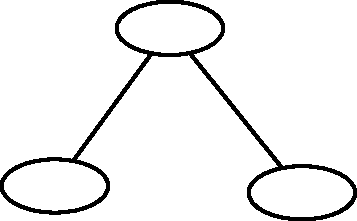
\includegraphics[width=.7\linewidth]{images/AVL0}
				\caption{AVL}
				\label{fig:avl0}
			\end{figure}
		\end{column}
		\begin{column}{0.33\textwidth}
			\begin{figure}
				\centering
				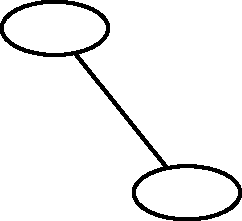
\includegraphics[width=.4\linewidth]{images/AVL1}
				\caption{AVL}
				\label{fig:avl1}
			\end{figure}
		\end{column}
		\begin{column}{0.33\textwidth}
			\begin{figure}
				\centering
				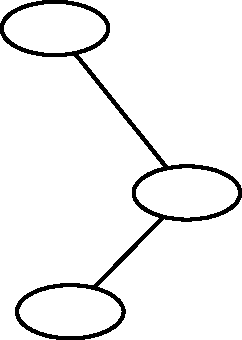
\includegraphics[width=.3\linewidth]{images/naoAVL}
				\caption{Não AVL}
				\label{fig:naoavl}
			\end{figure}
		\end{column}
	\end{columns}
\end{frame}

\begin{frame}
	\frametitle{Algoritmos de busca em grafos}
	\framesubtitle{AVL - Árvore de busca balanceada - Percurso em ordem}
	\par É uma forma de realizar um \textbf{percurso} na árvore binária. Um percurso é uma forma \textbf{sistemática} de percorrer os nós de uma árvore.
	\par No percuso em ordem o último elemento a ser exibido está sempre ao lado direito da raiz das árvores e sub-árvores e quando um elemento \textbf{não tem} filho a esquerda \textbf{que não foi mostrado} ele também é mostrado
	
	\only<1>{
		\begin{figure}
			\centering
			\includegraphics[width=0.7\linewidth]{images/arvoreBinaria2}
			\caption{Árvore binária}
			\label{fig:arvorebinaria3}
		\end{figure}
	}
	\only<2>{
		\par $G = \{d\}$
		\begin{figure}
			\centering
			\includegraphics[width=0.7\linewidth]{images/emordem0}
			\caption{Em ordem}
			\label{fig:emordem0}
		\end{figure}
	}
	\only<3>{
		\par $G = \{d,b\}$
		\begin{figure}
			\centering
			\includegraphics[width=0.7\linewidth]{images/emordem1}
			\caption{Em ordem}
			\label{fig:emordem1}
		\end{figure}
	}	
	\only<4>{
		\par $G = \{d,b,e\}$
		\begin{figure}
			\centering
			\includegraphics[width=0.7\linewidth]{images/emordem2}
			\caption{Em ordem}
			\label{fig:emordem2}
		\end{figure}
	}
	\only<5>{
		\par $G = \{d,b,e,a\}$
		\begin{figure}
			\centering
			\includegraphics[width=0.7\linewidth]{images/emordem3}
			\caption{Em ordem}
			\label{fig:emordem3}
		\end{figure}
	}
	\only<6>{
		\par $G = \{d,b,e,a,f\}$
		\begin{figure}
			\centering
			\includegraphics[width=0.7\linewidth]{images/emordem4}
			\caption{Em ordem}
			\label{fig:emordem4}
		\end{figure}
	}
	\only<7>{
		\par $G = \{d,b,e,a,f,c\}$
		\begin{figure}
			\centering
			\includegraphics[width=0.7\linewidth]{images/emordem5}
			\caption{Em ordem}
			\label{fig:emordem5}
		\end{figure}
	}
	\only<8>{
		\par $G = \{d,b,e,a,f,c,g\}$
		\begin{figure}
			\centering
			\includegraphics[width=0.7\linewidth]{images/emordem6}
			\caption{Em ordem}
			\label{fig:emordem6}
		\end{figure}
	}
\end{frame}

\begin{frame}
	\frametitle{Algoritmos de busca em grafos}
	\framesubtitle{AVL - Árvore de busca balanceada - Percurso pós-ordem}
	\par No percuso pós-ordem a raiz da árvore será o último nós a ser visitado, sendo assim, considerando que sub-árvores também tem suas raízes as mesmas terão, da mesma forma, suas raízes visitadas por último. Notou o padrão recursivo?
	
	\only<1>{
	\begin{figure}
		\centering
		\includegraphics[width=0.7\linewidth]{images/arvoreBinaria2}
		\caption{Árvore binária}
		\label{fig:arvorebinaria2}
	\end{figure}
	}
	\only<2>{
	\par $G = \{\emptyset\}$
	\begin{figure}
		\centering
		\includegraphics[width=0.7\linewidth]{images/posordem0}
		\caption{Pós-ordem}
		\label{fig:posordem0}
	\end{figure}
	}
	\only<3>{
	\par $G = \{\emptyset\}$
	\begin{figure}
		\centering
		\includegraphics[width=0.7\linewidth]{images/posordem1}
		\caption{Pós-ordem}
		\label{fig:posordem1}
	\end{figure}
	}	
	\only<4>{
	\par $G = \{d\}$
	\begin{figure}
		\centering
		\includegraphics[width=0.7\linewidth]{images/posordem2}
		\caption{Pós-ordem}
		\label{fig:posordem2}
	\end{figure}
	}
	\only<5>{
	\par $G = \{d,e\}$
	\begin{figure}
		\centering
		\includegraphics[width=0.7\linewidth]{images/posordem3}
		\caption{Pós-ordem}
		\label{fig:posordem3}
	\end{figure}
	}
	\only<6>{
	\par $G = \{d,e,b\}$
	\begin{figure}
		\centering
		\includegraphics[width=0.7\linewidth]{images/posordem4}
		\caption{Pós-ordem}
		\label{fig:posordem4}
	\end{figure}
	}
	\only<7>{
	\par $G = \{d,e,b\}$
	\begin{figure}
		\centering
		\includegraphics[width=0.7\linewidth]{images/posordem5}
		\caption{Pós-ordem}
		\label{fig:posordem5}
	\end{figure}
	}
	\only<8>{
	\par $G = \{d,e,b,f\}$
	\begin{figure}
		\centering
		\includegraphics[width=0.7\linewidth]{images/posordem6}
		\caption{Pós-ordem}
		\label{fig:posordem6}
	\end{figure}
	}
	\only<9>{
	\par $G = \{d,e,b,f,g\}$
	\begin{figure}
		\centering
		\includegraphics[width=0.7\linewidth]{images/posordem7}
		\caption{Pós-ordem}
		\label{fig:posordem7}
	\end{figure}
	}
	\only<10>{
	\par $G = \{d,e,b,f,g,c\}$
	\begin{figure}
		\centering
		\includegraphics[width=0.7\linewidth]{images/posordem8}
		\caption{Pós-ordem}
		\label{fig:posordem8}
	\end{figure}
	}
	\only<11>{
	\par $G = \{d,e,b,f,g,c,a\}$
	\begin{figure}
		\centering
		\includegraphics[width=0.7\linewidth]{images/posordem9}
		\caption{Pós-ordem}
		\label{fig:posordem9}
	\end{figure}
	}
\end{frame}

\begin{frame}
	\frametitle{Algoritmos de busca em grafos}
	\framesubtitle{AVL - Árvore de busca balanceada - Percurso pré-ordem - Exercício0}
	
	\par No percurso em pré-ordem sempre que a raíz de uma árvore ou sub-árvore é visitado o mesmo é exibido para em seguida se visitar o próximo nó a esquerda \textbf{até que não haja mais nós esquerdos}, depois disso se exibe os nós a direita.

	\par \textbf{Desenhe} o percurso da árvore binária em pré-ordem.
	\pause
	\par \textbf{Resposta:} $G = \{a,b,d,e,c,f,g\}$
	\begin{figure}
		\centering
		\includegraphics[width=0.7\linewidth]{images/preordem}
		\caption{Pré-ordem}
		\label{fig:preordem}
	\end{figure}
\end{frame}


\begin{frame}
	\frametitle{Algoritmos de busca em grafos}
	\framesubtitle{AVL - Árvore de busca balanceada - Algoritmos de percurso}
	\lstinputlisting[language=C++]{../codigo/percurso.cpp}
	
\end{frame}


\begin{frame}
	\frametitle{Algoritmos de busca em grafos}
	\framesubtitle{AVL - Árvore de busca balanceada - Algoritmo de balanceamento}
	\par Uma árvore binária, como já foi dito, pode degenerar em uma lista ligada sequencial prejudicando em muito o tempo de acesso aos seus dados. Para resolver isso se usa algumas técnicas de \textbf{rebalanceamento} da árvore.
\end{frame}

\begin{frame}
	\frametitle{Algoritmos de busca em grafos}
	\framesubtitle{AVL - Árvore de busca balanceada - Algoritmo de balanceamento}
	\begin{figure}
		\centering
		\includegraphics[width=0.7\linewidth]{images/AVLRotacaoAntiHoraria}
		\caption{Rotação anti-horária}
		\label{fig:avlrotacaoantihoraria}
	\end{figure}
	\begin{figure}
		\centering
		\includegraphics[width=0.7\linewidth]{images/AVLRotacaoHoraria}
		\caption{Rotação horária}
		\label{fig:avlrotacaohoraria}
	\end{figure}
\end{frame}

\begin{frame}
	\frametitle{Algoritmos de busca em grafos}
	\framesubtitle{AVL - Árvore de busca balanceada - Algoritmo de balanceamento}
	\par Baixe o código de \href{https://github.com/ensismoebius/1955SCC-Projeto-e-Analise-de-Algoritmos.git}{https://github.com/ensismoebius/1955SCC-Projeto-e-Analise-de-Algoritmos.git} e abra o projeto "arvoresEListas" lá você encontrará o arquivo \textit{main.cpp}. \textbf{Pergunta}: Qual o tempo de execução para adição e remoção de um item na AVL?
\end{frame}

\begin{frame}
	\frametitle{Algoritmos de busca em grafos}
	\framesubtitle{Árvores Trie}
	\par Uma Árvore Trie (termo definido em 1960 pelo professor Edward Fredkin a
	partir da abstração da palavra “retrieval”) pode ser descrita como uma estrutura de dados utilizada para armazenar de forma hierárquica cadeias de caracteres e suportar uma rápida procura de registros, sendo sua principal aplicação a procura por padrões	e prefixos. \newline
	\par O grande diferencial das Árvores Trie em relação as, por exemplo, árvores de busca binárias (ABB), é que o valor a ser armazenado (daqui em diante chamaremos esse valor de chave) não precisa ser totalmente guardado em alguma estrutura interna da árvore (nó), pois a própria estrutura da árvore Trie consegue representar senão	toda, boa parte da chave.
\end{frame}

\begin{frame}
	\frametitle{Algoritmos de busca em grafos}
	\framesubtitle{Árvores Trie}
	\par Organização dos dados em uma trie:
	\begin{itemize}
		\item dados não são guardados em apenas um nó
		\item dados são tratados como elementos divisíveis dispersos na árvore
		\item cada nó possui como valor implícito um caractere de um alfabeto pré-definido
		\item \textbf{prefixo de chave} é o caminho desde a raiz até um nó não-folha
	\end{itemize}
	\par O primeiro nível da trie é composto tão e somente por um único vetor, no qual é	colocado o primeiro caractere da chave que se pretende armazenar, caso a chave tenha mais de um caractere então será criado dinamicamente um outro vetor em um nível abaixo do primeiro, e, assim por diante até que todos os caracteres da chave	sejam mapeados.
\end{frame}

\begin{frame}
	\frametitle{Algoritmos de busca em grafos}
	\framesubtitle{Árvores Trie}
	\begin{columns}
		\begin{column}{0.7\textwidth}
			\begin{figure}
				\centering
				\includegraphics[width=\linewidth]{images/trie}
				\caption{Uma trie}
				\label{fig:trie}
			\end{figure}
		\end{column}
		\begin{column}{0.3\textwidth}
			\par Nós marcados em verde são as folhas da trie.
			\par Perceba que essa estrutura tem níveis.
			\par O que esses níveis tem de especial?
		\end{column}
	\end{columns}
\end{frame}

\begin{frame}
	\frametitle{Algoritmos de busca em grafos}
	\framesubtitle{Árvores Trie}
		\par Cada nó é representado usando uma estrutura como a abaixo:
		\begin{columns}
			\begin{column}{0.5\textwidth}
				\lstinputlisting[language=C++]{../codigo/trienode.h}
			\end{column}
			\begin{column}{0.5\textwidth}
				\lstinputlisting[language=C++]{../codigo/trienode.cpp}
			\end{column}
		\end{columns}
\end{frame}

\begin{frame}
	\frametitle{Algoritmos de busca em grafos}
	\framesubtitle{Árvores Trie}
	\par A trie com suas operações pode ser representada dessa forma:
	\lstinputlisting[language=C++]{../codigo/trie.h}
\end{frame}

\begin{frame}[allowframebreaks]
	\frametitle{Algoritmos de busca em grafos}
	\framesubtitle{Árvores Trie}
	\par A trie com suas operações pode ser representada dessa forma:
	\lstinputlisting[language=C++]{../codigo/trie.cpp}
\end{frame}


\begin{frame}
	\frametitle{Algoritmos de busca em grafos}
	\framesubtitle{Árvores Trie}
	\par \textbf{Exercício 1542660005445454545877:} Usando a trie crie um sistema que dado o \textbf{prefixo} de uma palavra o mesmo retorne todas as palavras cadastradas com aquele prefixo. Por exemplo: "par" $\rightarrow$ \textbf{par}angaricutirimiruaro, \textbf{par}aná, \textbf{par}cimônia, etc.
	\par Considerando que o tamanho da entrada $n$ é a quantidade de letras na palavra, qual o tempo de execução para \textbf{localizar uma palavra}?
	\par E quando a palavra não é encontrada?\newline
	\pause
	\par \textbf{Resposta}:
	\par $\Theta(n)$ e $O(n), \Omega(1)$
\end{frame}	
		
	\section{Análise de problemas P / NP}
		
\begin{frame}
	\frametitle{Análise de problemas P / NP}
	\par Inicialmente definiremos as classes de problemas P/NP para problemas de \textbf{decisão}, ou seja, problemas cujas respostas são \textbf{sim/não}
	
	\par No entanto, \textbf{pode ser} relativamente fácil converter um problema de otimização em um de decisão.
	
	\par \textbf{Por exemplo}:
	\par \textit{Existe um caminho de distância $K$ entre dois pontos de um grafo?} A resposta será sim ou não. \newline
	\par De forma mais genérica: Existe uma solução que satisfaz uma certa propriedade?\newline
	\par \textbf{No entanto} podemos estimar um valor para $K$ e ir perguntando ao algoritmo que, caso responda \textbf{não}, poderá responder sim para $K + j$ ou $K -j$ tal que $j$ seja um valor que faça com que exista uma solução. A forma de encontrar esse $j$ pode variar de acordo com a situação. Ou seja, associado a um problema de decisão pode estar vinculado um problema de \textbf{otimização}.
\end{frame}

\begin{frame}
	\frametitle{Análise de problemas P / NP}
	\framesubtitle{Algoritmos polinomiais}
	\par Algoritmos polinomiais são aqueles que podem ter seu \textbf{tempo representado na forma de um polinômio} de grau qualquer, basicamente quase todos os que vimos até agora,  por outro lado, algoritmos não polinomiais são aqueles cuja a representação é dada, por exemplo, por funções exponenciais.\newline
	\par A verdade é que não se pode ter \textbf{total certeza} que um algoritmo é não polinomial pois pode ser que, para um determinado problema, exista uma solução polinomial portanto, o que se pode afirmar é que \textbf{até o momento} se sabe que a solução desses problemas tem algoritmos de tempo não polinomial. 
\end{frame}

\begin{frame}
	\frametitle{Análise de problema P / NP}
	\framesubtitle{Algoritmos polinomiais}
	\par Dizemos que um algoritmo resolve um dado problema se, ao receber uma entrada do problema, devolve uma solução ou informa que não há solução.
	\par Se diz que um algoritmo é \textbf{razoavelmente rápido} quando o mesmo \textbf{tem um tempo polinomial}.
	\par Um algoritmo é polinomial se \textbf{o pior caso} do mesmo for algo como $O(n^i) \forall i \in  \mathbb{N}$
	\par Exemplos:
	\begin{itemize}
		\item $10n^3+3n^2+1 \implies O(n^3)$
		\item $n^5.\log n \leq n^6 \implies o(n^6)$
	\end{itemize}
	\par É importante separar os algoritmos polinomiais dos não polinomiais pois polinômios tem algumas características interessantes como fechamento em \textbf{adição, multiplicação e composição} que, quando aplicadas \textbf{não mudam} a natureza polinomial do tempo do algoritmo.
\end{frame}

\begin{frame}
	\frametitle{Análise de problemas P / NP}
	\framesubtitle{Algoritmos \textbf{não} polinomiais}
	\par São todos aqueles que consomem um tempo \textbf{não polinomial} como, por exemplo, $e^n$, $n!$, $2^n$, etc.
	\par Geralmente a resolução desses problemas é custosa e se dá pela estratégia da \textbf{força bruta}. É verdade que, ainda assim, é possível economizar alguns ciclos de processamento usando uma \textbf{árvore de estados} mas isso não muda o tempo assintótico do algoritmo.
\end{frame}

\begin{frame}
	\frametitle{Análise de problemas P / NP}
	\framesubtitle{A classe P de problemas}
	\par A classe $P$ de problemas compreende todos os algoritmos que podem ser executados em um tempo polinomial, \textbf{o fato de ainda não se ter encontrado um algoritmo polinomial para um problema não garante \textit{definitivamente} que a natureza do problema seja não polinomial}.
\end{frame}

\begin{frame}
	\frametitle{Análise de problemas P / NP}
	\framesubtitle{O problema da satisfazibilidade  (S.A. Cook, L.A. Levin, 1973)}
	\par Dada uma fórmula booleana na forma normal \textbf{conjuntiva} ou \textbf{disjuntiva}. Existem valores para $x_1,x_2,x_3, \dots x_n$ que resultam em \textbf{Verdadeiro} para essa fórmula?
	\par Exemplos de instâncias:
	\begin{enumerate}
		\item conjuntiva: $(x_1 \vee \neg x_2)\wedge(x_1 \vee x_3)\wedge(\neg x_1 \vee x_2)$ \label{enum:conj}
		\item disjuntiva: $(x_1 \wedge \neg x_2)\vee(x_1 \wedge x_3)\vee(\neg x_1 \wedge x_2)$\label{enum:disjun}
	\end{enumerate}
	\par À \textbf{solução} dessa fórmula daremos o nome de \textbf{certificado}.
	\par O \textbf{certificado} garante que, dado o problema, teremos a resposta \textbf{sim}. De outra forma: O certificado é a \textbf{prova} de que a resposta sim é verdadeira.
	\par Para o exemplo \ref{enum:conj} o certificado é $x_1=Verdadeiro, x_2=Verdadeiro$\newline
	
	\par \textbf{Pergunta}: Existe um \textbf{certificado} para o problema \ref{enum:disjun}? Qual?
	
	\par Considerando o problema da satisfazibilidade entremos no campo dos problemas \textbf{NP}. Mais especificamente \textbf{NP-completo}.
\end{frame}

\begin{frame}
	\frametitle{Análise de problemas P / NP}
	\framesubtitle{A classe NP de problemas}
	\par A classe $NP$ é aquela dos algoritmos não polinomiais certo? \textbf{Errado!}
	\par \textbf{NP} é um acrônimo para \textit{Non-deterministic polynomial time}, ou seja, é uma classe de problemas cuja validade de um certificado pode ser avaliada em tempo \textbf{polinomial} e cuja a solução pode ser obtida em tempo polinomial usando um sistema de computação \textbf{hipotético} não determinístico (o que se aproxima mais disso são os atuais computadores quânticos).
	\par De outra forma: Dada uma solução hipotética para um problema NP é rápido e fácil (tempo polinomial) verificar se aquela solução é \textbf{verdadeira}. Já, descobrir uma solução para o problema, bom... aí é outra estória pois esse tipo de problema \textbf{não tem algoritmos conhecidos} cujo tempo de geração de um certificado seja polinomial.
	\par Daí tiramos que $P \subset NP$.
	\par Obs: \textbf{Não se sabe} se $P = NP$ ou não, quem conseguir provar isso (que $P = NP$ ou  $P \neq NP$) revolucionará a área da computação.	
\end{frame}

\begin{frame}
	\frametitle{Análise de problemas P / NP}
	\framesubtitle{A classe NP de problemas}
	\par Considerando que qualquer problema que possa, de alguma forma, ser transformado no problema da satisfazibilidade ou em qualquer outro problema NP \textbf{também é NP}, afim de provar que $P=NP$ ou $P \neq NP$ basta provar isso para \textbf{um} único problema $NP$!
	\newline
	\par A página do professor \textit{Paulo Feofiloff} tem muitos exemplos:
	\href{https://www.ime.usp.br/~pf/analise_de_algoritmos/aulas/NPcompleto.html}{https://www.ime.usp.br/\texttildelow pf/analise\_de\_algoritmos/aulas/NPcompleto.html} 
\end{frame}

\begin{frame}
	\frametitle{Análise de problemas P / NP}
	\framesubtitle{Redução polinomial}
	\par Da definição anterior tiramos que: Seja $A$ um problema e $B$ outro cuja solução é conhecida. Se a conversão de $A$ para $B$ é possível então solucionar $A$ também o será.
	\par Ao procedimento descrito acima damos o nome de redução polinomial de $A$ para $B$ ou $A \preceq B$ (lê-se A é redutível a B) onde $B$ é um algoritmo polinomial
	\par É importante dizer que $B\subseteq A$ e $B$ pode ser chamado múltiplas vezes em $A$.\newline
	
	\par \textbf{Exemplo}: \textit{Selecione o enésimo termo de uma sequência numérica randômica.}
	\par Tal problema pode ser reduzido a uma de ordenação seguida de uns poucos comandos.	
	
	\par Sendo assim, suponha que $A \preceq B$ então:
	\begin{itemize}
		\item se $B \in P \implies A \in P$
		\item se $B \preceq C \implies A \preceq C$
		\item se $B \in P \implies A \in P$
		\item se $B \in NP$ \textbf{talvez} haja uma solução de $A \in P$ que não use $B$.
		\item se $A$ não tem solução polinomial e $A \preceq B / B \in NP \implies A \in NP$
	\end{itemize}
\end{frame}

\begin{frame}
	\frametitle{Análise de problemas P / NP}
	\framesubtitle{Redução polinomial - NP-completo}
	\par \textbf{Então} se $\mathbf{NP-completo} \subset NP, A \in NP, B \preceq A \forall B \in NP \implies A \in \mathbf{NP-completo}$\newline
	\par Embora NP (e NP-completo) de tenha como domínio os problemas de decisão, \textbf{como ja vimos} existe uma correlação entre problemas de otimização e de decisão que garante que o problema de decisão correspondente ao de otimização deve ser pelo menos \textbf{não mais difícil} que o de otimização. 
	\par De outra forma: Se um problema de otimização é polinomial sua respectiva decisão também o será, \textbf{o inverso não é necessariamente verdade}.
	
	\par \textbf{Finalmente} problemas NP-completos são aqueles que podem de alguma forma serem reduzidos ao problema da satisfazibilidade (meh...)
\end{frame}

\begin{frame}
	\frametitle{Análise de problemas P / NP}
	\framesubtitle{Exercício 0}
	\par Crie um programa que:
	\begin{itemize}
		\item verifique se um número é primo ou não
		\item gere o enésimo numero primo dado um valor de $n$
	\end{itemize}
	\par \textbf{Determine o tempo de execução de ambos}
	\par \textbf{Algum dos dois é NP?}
	\par \textbf{Qual a relação entre eles?}
\end{frame}

\begin{frame}
	\frametitle{Análise de problemas P / NP}
	\framesubtitle{Exercício 1}
	\begin{itemize}
		\item Determine um circuito hamiltoniano de custo mínimo.
		\item Dado um valor $L$ existe um circuito de custo $L$?
	\end{itemize}
	\par \textbf{Determine o tempo de execução de ambos}
	\par \textbf{Algum dos dois é NP?}
	\par \textbf{Qual a relação entre eles?}\newline
	
	\par Um \textit{circuito hamiltoniano} é um circuito/ciclo cujos elementos não se repetem.
\end{frame}

\begin{frame}
	\frametitle{Análise de problemas P / NP}
	\framesubtitle{Exercício 2}
	\begin{itemize}
		\item Determine quantas cliques com 2 e 3 elementos um certo grafo pode ter.
		\item Dado uma quantidade e elementos $k$ existe um clique com $k$ elementos?
	\end{itemize}
	\par \textbf{Determine o tempo de execução de ambos}
	\par \textbf{Algum dos dois é NP?}
	\par \textbf{Qual a relação entre eles?}\newline
	
	\par Uma \textit{clique} é um subgrafo completo.
\end{frame}

\begin{frame}
	\frametitle{Análise de problemas P / NP}
	\framesubtitle{Exercício 3}
	\begin{itemize}
		\item Dado um grafo o mesmo é euleriano?
	\end{itemize}
	\par \textbf{Determine o tempo de execução}
	\par \textbf{Esse algoritmo é NP?}\newline
	
	\par Um grafo euleriano é aquele em que é possível percorrer todas as arestas do mesmo podendo apenas repetir os vértices. Grafos eulerianos tem todos os vértices com grau par.
\end{frame}

\begin{frame}
	\frametitle{Análise de problemas P / NP}
	\framesubtitle{Exercício 4}
	\par Considere $S \subseteq \mathbb{Z} / k \in S, |S| = n, n \in \mathbb{N}$, ou seja, $S$ é subconjunto de $\mathbb{Z}$ e a quantidade de elementos de $S$ é igual a um $n$ qualquer natural, então: Existe $\sum_{i \in S} k_i = \sum_{i \notin S} k_i$?
\end{frame}

		
	\section{Algoritmos de força bruta}
		\begin{frame}
	\frametitle{Algoritmos de força bruta}
	\begin{figure}
		\centering
		\includegraphics[width=.9\linewidth]{images/bodyBuildPorra}
		\caption{Processei pra crl! Vai dar sim!}
		\label{fig:bodybuildporra}
	\end{figure}
	
\end{frame}

\begin{frame}
	\frametitle{Algoritmos de força bruta}
	\par São aqueles cuja a definição não se pode expressar em termos polinomiais ou cujos tempos são muito grandes, geralmente são feitos para mapear todas as opções dentro de um certo espaço de procura resultando assim em ordens de tempo muito grandes.
	
	\par Geralmente tais algoritmos estão ligados a um pensamento mais direto de resolução do problema e dependente do poder de processamento do computador e não da inteligência na modelagem.\newline
	
	\par Alguns dos exemplos que já vimos são o \textbf{burbble-Sort}, \textbf{Selection-Sort}, além de outros como \textbf{Busca sequencial}, \textbf{multiplicação de matrizes}, etc.\newline
	
	\par No entanto, existem técnicas como o \textbf{bactracking} ou \textbf{retro-rastreamento} e \textbf{branching-and-bound} ou \textbf{ramificar e limitar} que são estratégias que usam uma \textbf{árvores de estados} e podem melhorar um pouco tais tempos de execução.	
\end{frame}

\begin{frame}
	\frametitle{Algoritmos de busca em grafos}
	\framesubtitle{Árvore de estados}
	\par Esta árvore indica em cada um dos seus nós um estado alcançado pelo sistema, assim, é possível, considerando-se certas condições, julgar a possibilidade ou a utilidade de se fazer novos testes, ou ainda, se é necessário voltar a algum estado anterior. Existem técnicas como o \textbf{backtracking} ou \textbf{retro-rastreamento} e \textbf{branching-and-bound} ou \textbf{ramificar e limitar} que são estratégias que usam uma \textbf{árvores de estados} e podem melhorar um pouco os tempos de execução de algoritmos de força bruta.
	
	\tikzset{
		tree/.style={
			every node/.style={rectangle,draw},
			level 1/.style={sibling distance=60mm},
			level 2/.style={sibling distance=30mm},
			level 3/.style={sibling distance=20mm},
		},
		fontbf/.style={font=\bfseries}
	}
	
	\begin{figure}
		\begin{tikzpicture}[tree]
			\node {E1}
			child{
				node{E1 + E2}
				child{node{E1 + E2 + E4}}
				child{node{E1 + E2 + E5}}
			}
			child{
				node{E1 + E3}
				child{node{E1 + E2 + E6}}
				child{node{E1 + E2 + E7}}
			};
		\end{tikzpicture}
	\end{figure}
\end{frame}

\begin{frame}
	\frametitle{Algoritmos de força bruta}
	\framesubtitle{Retro-rastreamento - Ramificar e limitar}
	\par Dado um problema de otimização, se o custo de uma solução possível ultrapassou o valor de outra então se pode parar como o processamento daquela possibilidade.
		\begin{columns}
		\begin{column}{0.5\textwidth}
			\begin{figure}
				\centering
				\includegraphics[width=0.8\linewidth]{images/grafoForcaBruta}
				\caption{Caixeiro viajante}
				\label{fig:grafoforcabruta}
			\end{figure}
		\end{column}
		\begin{column}{0.5\textwidth}
			\begin{figure}
				\centering
				\includegraphics[width=0.8\linewidth]{images/arvoreEstadoForcaBruta}
				\caption{Árvore de estados}
				\label{fig:arvoreestadoforcabruta}
			\end{figure}
		\end{column}
	\end{columns}
\end{frame}

\begin{frame}
	\frametitle{Algoritmos de força bruta}
	\framesubtitle{Retro-rastreamento - Ramificar e limitar - Exercício}
	\par Posicione 4 rainhas em um tabuleiro 4x4 sem que elas se ataquem. Monte a árvore de estados com Retro-rastreamento e Ramificar e limitar.
\end{frame}
	
	%\begin{frame}[allowframebreaks]
	%	\frametitle{Referências}
	%	\bibliography{bibliography.bib}
	%\end{frame}
	
\end{document}